% 2012-10-08 toph This document stared as a copy paste from
%                 /usr/share/doc/latex-beamer/solutions/conference-talks/conference-ornate-20min.en.tex
%                 which is a template created by Till Tantau 
%                 in 2004.
% -----------------------------------------------------------

\documentclass[9pt,xcolor={dvipsnames}]{beamer}
%\documentclass[9pt,xcolor={dvipsnames},handout]{beamer}
%
%2013-11-18 toph   'xcolor={dvipsnames}' gives me access to WAY
%                   more colors

\mode<presentation>
{
  \usetheme{Warsaw}
  % or ...

  \setbeamercovered{transparent}
  % or whatever (possibly just delete it)
}


\usepackage[english]{babel}
% or whatever

\usepackage[latin1]{inputenc}
% or whatever
%\usepackage[usenames,dvipsnames]{color}
\usepackage{multimedia}
\usepackage{times}
\usepackage[T1]{fontenc}
% Or whatever. Note that the encoding and the font should match. If T1
% does not look nice, try deleting the line with the fontenc.

\expandafter\def\expandafter\insertshorttitle\expandafter{%
\insertshorttitle\hfill%
\insertframenumber\,/\,\inserttotalframenumber}

%2013-10-15  toph  Created this file as a one-stop-shop for
%                  all of my custom commands... I really need
%                  TO COMMENT ANY CHANGES OR ADDITIONS
%
%2013-10-15  toph  added shorter \rSp{} since I use \realSpace{}
%                  all the time
%2013-10-16  toph  added the eig math operator
%2013-10-21  toph  added the regressor new commands e.g. \UVreg
%2013-10-31  toph  added space 0(3) 
%2013-11-3   toph  added the math operator e
%2013-11-4   toph  added cross operator in the heat of battle
%------------------------------------------------------------
%-----------------COMMENT ANY CHANGES OR ADDITIONS-----------
\DeclareMathOperator{\cross}{cross}
\DeclareMathOperator{\O3}{O(3)}
\DeclareMathOperator{\SE3}{SE(3)}
\DeclareMathOperator{\SO3}{SO(3)}
\DeclareMathOperator{\se3}{se(3)}
\DeclareMathOperator{\so3}{so(3)}
\DeclareMathOperator{\e}{e}
\DeclareMathOperator{\id}{id}
\DeclareMathOperator{\sgn}{sgn}
\DeclareMathOperator{\tr}{tr}
\DeclareMathOperator{\ad}{ad}
\DeclareMathOperator{\Ad}{Ad}
\DeclareMathOperator{\eig}{eig}
\newcommand{\minNorm}[1]{\|#1\|_{\text{min}} }
\newcommand{\soThreeMap}[1]{\mathcal{J}\left( #1 \right)}
\newcommand{\realSpace}[1]{\mathbb{R}^{#1}}
\newcommand{\rSp}[1]{\realSpace{#1}}
\newcommand{\funDefn}[3]{$#1 : #2 \to #3$}
\newcommand{\OKCg}{\mathfrak{g}}
\newcommand{\OKCpos}{q}
\newcommand{\OKCinput}{\tau}
\newcommand{\Ireg}{\mathbb{W}_{I}}
\newcommand{\Mreg}{\mathbb{W}_{M}}
\newcommand{\Dreg}[1]{\mathbb{W}_{D #1}}
\newcommand{\gbreg}{\mathbb{W}_{gb}}
\newcommand{\UVreg}{\mathbb{W}_{UV}}
\newcommand{\UVregStack}{\mathcal{W}_{UV}}
\newcommand{\UVRreg}{\mathbb{W}_{UVR}}
\newcommand{\UVRregStack}{\mathcal{W}_{UVR}}
\newcommand{\OKCreg}{\mathbb{W}_{OKC}}
\newcommand{\OKCparam}{\theta_{OKC}}
\newcommand{\OKCparamDot}{\dot{\theta}_{OKC}}
\newcommand{\OKCparamEst}{\hat{\theta}_{OKC}}
\newcommand{\OKCparamEstDot}{\dot{\hat{\theta}}_{OKC}}
\newcommand{\OKCparami}{\theta_{OKCi}}
\newcommand{\MBCreg}{\mathbb{W}_{MBC}}
\newcommand{\MBCregi}{\mathbb{W}_{MBC_i}}
%-----------------COMMENT ANY CHANGES OR ADDITIONS-----------
%------------------------------------------------------------


\title[UV Adaptive Identification and Control] % (optional, use only with long paper titles)
{Adaptive Identification and Control of Underwater Vehicles:\\ Theory and Comparative Experimential Evaluation}

%\subtitle
%{Include Only If Paper Has a Subtitle}

\author[McFarland] % (optional, use only with lots of authors)
{C. J. ~McFarland}
% - Give the names in the same order as the appear in the paper.
% - Use the \inst{?} command only if the authors have different
%   affiliation.

\institute[Johns Hopkins University] % (optional, but mostly needed)
{
  %\inst{1}%
  Mechanical Engineering Department \\
  Johns Hopkins University
  %\and
  %\inst{2}%
  %Department of Theoretical Philosophy\\
  %University of Elsewhere
}
% - Use the \inst command only if there are several affiliations.
% - Keep it simple, no one is interested in your street address.

\date%[ICRA 2013] % (optional, should be abbreviation of conference name)
{Dissertation Defense}
% - Either use conference name or its abbreviation.
% - Not really informative to the audience, more for people (including
%   yourself) who are reading the slides online

%\subject{Theoretical Computer Science}
% This is only inserted into the PDF information catalog. Can be left
% out. 



% If you have a file called "university-logo-filename.xxx", where xxx
% is a graphic format that can be processed by latex or pdflatex,
% resp., then you can add a logo as follows:

% \pgfdeclareimage[height=0.5cm]{university-logo}{university-logo-filename}
% \logo{\pgfuseimage{university-logo}}



% Delete this, if you do not want the table of contents to pop up at
% the beginning of each subsection:
%\AtBeginSubsection[]
%{
%  \begin{frame}<beamer>{Outline}
%    \tableofcontents[currentsection,currentsubsection]
%  \end{frame}
%}


% If you wish to uncover everything in a step-wise fashion, uncomment
% the following command: 

%\beamerdefaultoverlayspecification{<+->}


\begin{document}



\begin{frame}
  \titlepage
\end{frame}

\begin{frame}{Outline}

  \tableofcontents
  % You might wish to add the option [pausesections]

\end{frame}

% \begin{frame}{Outline}
% \begin{columns}
% \column{.5\textwidth}
%   \tableofcontents
%   % You might wish to add the option [pausesections]
% \column{.5\textwidth}
%   \begin{center}
% \begin{figure}[htbp]  
%   \begin{center}
%     \movie[width=40mm]{placeholder box}{6dofid_vid.avi}
%     %\includegraphics[]{}
%   \end{center}
%   %\caption{McFarland and Nereus (WHOI) during field deployment in 2011.}
% \end{figure}
% \end{center}

% \end{columns}

% \end{frame}

% \begin{frame}{temporalTest}
% \begin{itemize}
%   \item<1-> stuff
%   \item<2-> about
%   \item<3-> rigid body
% \end{itemize}
% \temporal<2>
% {

% one

% }{

% two

% }{

% three}
% \end{frame}

% Structuring a talk is a difficult task and the following structure
% may not be suitable. Here are some rules that apply for this
% solution: 

% - Exactly two or three sections (other than the summary).
% - At *most* three subsections per section.
% - Talk about 30s to 2min per frame. So there should be between about
%   15 and 30 frames, all told.

% - A conference audience is likely to know very little of what you
%   are going to talk about. So *simplify*!
% - In a 20min talk, getting the main ideas across is hard
%   enough. Leave out details, even if it means being less precise than
%   you think necessary.
% - If you omit details that are vital to the proof/implementation,
%   just say so once. Everybody will be happy with that.

\section{Introduction}
\subsection{Motivation}
\begin{frame}[t]{Motivation}
  Recent advances in Underwater Vehicle (UV) systems have enabled
  scientists and engineers to consider complex, multifaceted UV
  missions previously thought impractical or infeasible.

\uncover<6->{  \alert{Thesis Goal}: Develop improved
  {\bf state estimation}, {\bf parameter identification}, and
  {\bf control} algorithms.}
%    
    \begin{columns}
      \column{.45\textwidth}
\alt<1>{}{    \begin{center}
      \begin{figure}[htbp]
        \begin{center}
          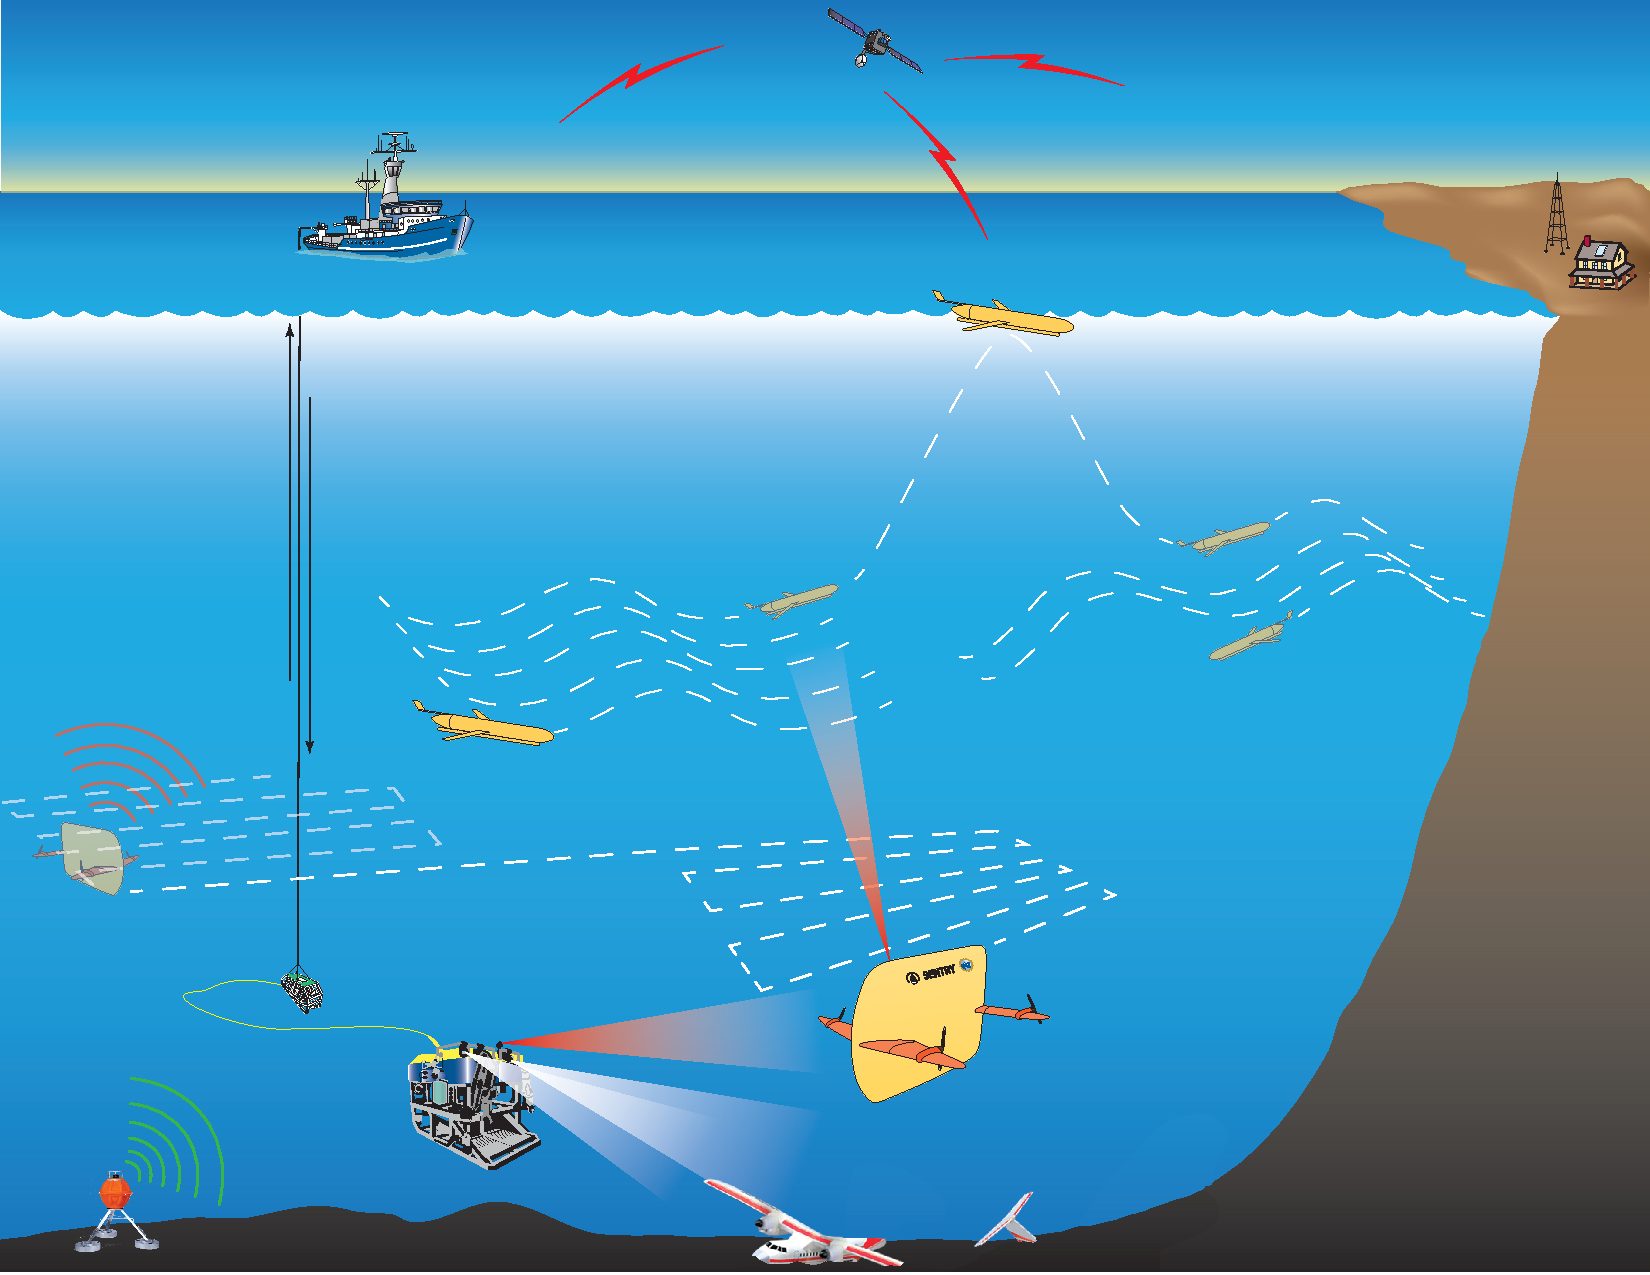
\includegraphics[width=1.1\textwidth]{./pres/images/Adaptive4}
%\caption{ Image credit: Paul Oberlander, WHOI. }
        \end{center}
      \end{figure}
    \end{center}
{\small Image credit: Paul Oberlander, WHOI.}}

  \column{.55\textwidth}

\alt<1-5>{
  \begin{itemize}
  \item<3-> UV teams for environmental monitoring
  \item<4-> Ship-based or on-shore operator monitoring and re-tasking of
    UVs
  \item<5-> Deployment of UVs in delicate or dynamic environments
  \end{itemize}
}{
  \begin{itemize}
  \item<7-> {\bf Improved State Estimation} algorithms can
    increase navigation accuracy while lowering UV cost.
  \item<8-> {\bf Improved Parameter Identification} algorithms enable
    remote operators to use forward simulation for mission planning
    and diagnose UV failure.
  \item<9-> {\bf Improved Control} algorithms enable increased precision
    of delicate or dynamic 6-degree-of-freedom
    (DOF) operation.
  \end{itemize}
}

 \end{columns}

\end{frame}

\subsection{Thesis Contributions}
\begin{frame}{Thesis Contributions}

{\small
{\setbeamercolor*{item}{fg=blue}
   \begin{columns}
      \column{.32\textwidth}
{\color{blue} \bf State Estimation:}
    \begin{center}
      \begin{figure}[t!]
        \begin{center}
          
\includegraphics[width=\textwidth]{./pres/images/justGliders}
        \end{center}
      \end{figure}
    \end{center}
  \column{.75\textwidth}
%{\fontsize{7}{11}\selectfont
   \begin{itemize}
\item<1> 3-DOF Rotational Plant Velocity Observer %with stability analysis
\item<1> Simulation Study: 3-DOF Rotational Plant Velocity Observers
   \end{itemize}%}
\end{columns}}

{\color{OliveGreen}\rule{\linewidth}{4pt}
\setbeamercolor*{item}{fg=OliveGreen}
\vspace*{-5mm}
   \begin{columns}
      \column{.32\textwidth}
{\bf Parameter Identification:}
 %   \begin{center}
      \begin{figure}[t!]
        \begin{center}
          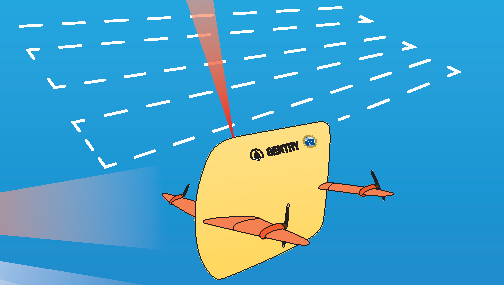
\includegraphics[width=\textwidth]{./pres/images/justSentry}
        \end{center}
      \end{figure}
%    \end{center}
  \column{.75\textwidth}
%{\tiny
\begin{itemize}
\item 3-DOF Rotational Dynamics Adaptive Identification (AID)
\item<1> Simulation Study: 3-DOF Rotational Plant AID
\item<1> {\it n}-link Open Kinematic Chain AID 
\item<1> 3-DOF UV Rotational Dynamics AID
\item<1> Experimental Evaluation: 3-DOF UV Rotational Dyn. AID
\item 6-DOF UV AID
\item Experimental Evaluation: 6-DOF UV AID
   \end{itemize}%}
\end{columns}}

{\color{red}\rule{\linewidth}{4pt}
\setbeamercolor*{item}{fg=red}
\vspace*{-2mm}
   \begin{columns}
      \column{.32\textwidth}
{\bf Trajectory-Tracking:}
    \begin{center}
      \begin{figure}[htbp]
        \begin{center}
          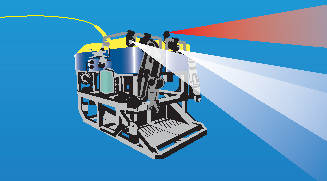
\includegraphics[width=\textwidth]{./pres/images/justJason}
        \end{center}
      \end{figure}
    \end{center}
  \column{.75\textwidth}
%{\tiny
\vspace*{-2mm}
   \begin{itemize}
\item 6-DOF UV Model-Based Control (MBC)
\item 6-DOF UV Adaptive Model-Based Control (AMBC)
\item Experimental Analysis: Thruster Dynamics and AMBC
\item<1> Two-Step UV AMBC
\item<1-2> Experimental Evaluation: UV Two-Step AMBC
   \end{itemize}%}
\vskip9pt
\end{columns}}}

\end{frame}

\section{Adaptive Parameter Identification}

\begin{frame}[t]{Adaptive Identification, Overview}%{LS Model Identification}

   \begin{columns}
      \column{.40\textwidth}
 %   \begin{center}
      \begin{figure}[t!]
        \begin{center}
          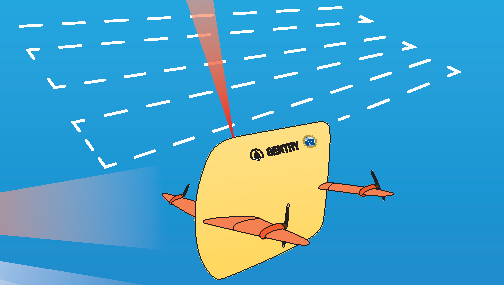
\includegraphics[width=\textwidth]{./pres/images/justSentry}
        \end{center}
      \end{figure}
%    \end{center}
  \column{.60\textwidth}

   \begin{itemize}
\item \alert<7>{Standard Model for Underwater Vehicle Dynamics}
\item<1-6> 3-DOF Rotational Dynamics Adaptive Identification (AID) Stability Analysis
\item<1-6> 6-DOF UV AID Algorithm
\item<1-6> Experimental Evaluation: 6-DOF UV AID
   \end{itemize}
\end{columns}
\vskip9pt
\alt<1-4>{
\pause
Previous Research into UV Parameter Identification:
\pause
\begin{itemize}
\item Most previously reported studies used conventional least squares identification (LS).
\begin{itemize}
\item LS requires UV acceleration to be instrumented; this signal is
  frequently not instrumented.
\end{itemize}
\pause
\item Previously reported adaptive methods were Adaptive Model-Based
  Controllers (AMBCs). These are not applicable when
\begin{itemize}
\item UV is uncontrolled,
\item under open-loop control, or
\item using any control law other than a specific trajectory-tracking AMBC.
\end{itemize}
\end{itemize}}
{
\uncover<5-6>{
\begin{itemize}
 \item<5-6> Adaptive identification algorithms do not require simultaneous
    reference trajectory-tracking control, nor do they require
    instrumentation of linear acceleration or angular acceleration;
  \item<6> Together, these facts make adaptive identification applicable
    to a wider class of UVs than previously reported methods.
  \end{itemize}
}
}
\end{frame}


\subsection{Standard Underwater Vehicle (UV) Model}

\begin{frame}[t]{Standard Underwater Vehicle (UV) Model}%{LS Model Identification}
 \begin{align} 
   \dot{H}(t)&=\underbrace{H(t)\widehat{v(t)}}_{\text{Kinematics}}
   \nonumber \\
   \underbrace{M\dot{v}(t)}_{\text{Inertial}}&=\underbrace{\ad_{v(t)}^TM v(t)}_{\text{Coriolis}}
   +\underbrace{\sum_{i=1}^6 |v_i |D_i v(t)}_{\text{Drag}} 
   +\underbrace{\mathcal{G}(g,b,H(t))}_{\text{Gravitational}}
   +\underbrace{u(t)}_{\text{Input}}
   \nonumber
\end{align}

\end{frame}


\begin{frame}[t]{Standard Underwater Vehicle (UV) Model}%{LS Model Identification}
 \begin{align} 
   \dot{H}(t)&={\color<3>{cyan}H(t)}\widehat{\color<3>{cyan} v(t)}
   \nonumber \\
   \alert<4-5>{M}\dot{v}(t)&=\ad_{\color<3>{cyan} v(t)}^T\alert<4-5>{M}{\color<3>{cyan} v(t)}  +
   \sum_{i=1}^6 |{\color<3>{cyan}v_i} |\alert<4-5>{D_i}
            {\color<3>{cyan}v(t)}+
   \mathcal{G}(\alert<4-5>{g},\alert<4-5>{b},{\color<3>{cyan}H(t)})+\color<2>{green}u(t)
   \nonumber 
 \end{align}


 \alt<1-4>{ 
    \begin{columns}
      \column{.55\textwidth}
      \pause
 %     \pause
      \color<2>{green}{Plant Input}
      
      \begin{itemize}
      \item
        ${\color<2>{green}u(t)}\in \mathbb{R}^6$ control force and torque
      \end{itemize}

      \vskip5pt plus.5fill

      \pause

      \color<3>{cyan}{Plant States}
      
      \begin{itemize}
      \item
        ${\color<3>{cyan}H(t)}\in \SE3$ pose

        (position and orientation)
      \item
        ${\color<3>{cyan}v(t)}\in \mathbb{R}^6$  velocity

        (body frame translational and angular velocities)
      \end{itemize}

      \column{.45\textwidth}


      

     \pause 
     \alert<4>{Parameters} (241 scalar parameters)
      \begin{itemize}
      \item
        ${\alert<4> M}\in \mathbb{R}^{6\times 6}$ sum of vehicle and
        hydrodynamic mass 
        
        (21 scalar parameters)
      \item
        $\alert<4>{D_i}\in \mathbb{R}^{6\times 6}$ Drag 
        
        (216 scalar parameters)  
      \item
        ${\alert<4> b}\in \mathbb{R}^{3}$ Buoyancy torque 
        
        (3 scalar parameters)
      \item
        ${\alert<4> g}\in \mathbb{R}$ Gravitational force 
        
        
        (1 scalar parameter)
      \end{itemize}

    \end{columns} 
  }
  {
    \begin{itemize}
    \item<5-> Parameters enter linearly into UV Model
      % \item<9-> $W:\mathbb{R}^3\times\mathbb{R}^3\times\SE3
      %   \to\mathbb{R}^{36\times 3}$ is a regressor matrix
    \item<6-> LS estimate of parameters possible, requires signals 
      $\{\dot{v}(t),v(t),H(t),u(t)\}$
    \item<7-> vehicle acceleration, $\dot{v}(t)$, is typically not instrumented  
    \item<8-> Adaptive Identification does not require $\dot{v}(t)$
    \end{itemize}
  }

\end{frame}



%\subsection{Rotating Rigid Body Model}

\begin{frame}[t]{A Simpler Model\dots Rotating Rigid Body}%{LS Model Identification}

Standard Underwater Vehicle (UV) Model
  
  \begin{align} 
   \dot{H}(t)&=\underbrace{H(t)\widehat{v(t)}}_{\text{Kinematics}}
   \nonumber \\
   \underbrace{M\dot{v}(t)}_{\text{Inertial}}&=
   \underbrace{\ad_{v(t)}^TM v(t)}_{\text{Coriolis}}
   \uncover<1>{+\underbrace{\sum_{i=1}^6 |v_i |D_i v(t)}_{\text{Drag}} 
   +\underbrace{\mathcal{G}(g,b,H(t))}_{\text{Gravitational}}}
   +\underbrace{u(t)}_{\text{Input}}
   \nonumber
\end{align}
\pause

Rotating Rigid Body Model

\begin{align} 
    \dot{R}(t)&=\underbrace{R(t)\mathcal{J}(\omega(t))}_{\text{Kinematics}}
    \nonumber \\
    \underbrace{I\dot{\omega}(t)}_{\text{Inertial}}&=\underbrace{\mathcal{J}(I\omega(t))\omega(t)}_{\text{Coriolis}}
    +\underbrace{\tau(t)}_{\text{Input}}
    \nonumber
  \end{align}

  \pause
  
            {\tiny  
                 C. J. McFarland and L. L. Whitcomb. A New Adaptive
                Identifier for Second-Order Rotational Plants with
                 Applications to Underwater Vehicles.  In OCEANS,
                   2012. Proceedings of MTS/IEEE, pages 1-9, Hampton
                 Roads, VA, 2012}


\end{frame}


%\begin{frame}[t]{Rigid Body Model}
%  \begin{align} 
%    \uncover<1>{\dot{R}(t)}&\uncover<1>{=R(t)\mathcal{J}(\omega(t))}
%    \nonumber \\
%    I\dot{\omega}(t)&=\mathcal{J}(I\omega(t))\omega(t)
%    \uncover<1>{+\left(\sum_{i=1}^3 |\omega_i|C_i
%    \right)\omega(t)+\mathcal{J}(b)R(t)^T e_3}+u(t)
%    \nonumber 
% \end{align}
%
% \begin{itemize}
%   \item<2-> Standard Second Order Rotating Rigid Body System 
%   \item<3-> Typically used to model satellites
%   \item<4-> We first developed an Adaptive Identifier for this system first
% \end{itemize}
%
%\end{frame}


%\begin{frame}[t]{Rotating Rigid Body Model}%{LS Model Identification}
%  Second-Order Rotational Plant Model
%  
%  \begin{align} 
%    \dot{R}(t)&=\underbrace{R(t)\mathcal{J}(\omega(t))}_{\text{Kinematics}}
%    \nonumber \\
%    \underbrace{I\dot{\omega}(t)}_{\text{Inertial}}&=\underbrace{\mathcal{J}(I\omega(t))\omega(t)}_{\text{Coriolis}}
%    +\underbrace{\tau(t)}_{\text{Input}}
%    \nonumber
%  \end{align}
%
%  
%
%\uncover<2->{
%  \begin{columns}
%  \column{.45\textwidth}
%\begin{itemize}
%  \item  $I\in\mathbb{R}^{3 \times 3}$ Positive Definite Symmetric Moment of Inertia
%  \item  $\omega\in\mathbb{R}^{3}$ Angular Velocity
%\end{itemize}
%
%\column{.55\textwidth}
%
%\begin{equation*}
%\mathcal{J}\left(
%\left[ \begin{array}{c} 
%\omega_1 \\\omega_2  \\ \omega_3 \\
%\end{array} \right]\right) =
%\left[ \begin{array}{ccc}
%     0     & -\omega_3 &  \omega_2                               \\
%   \omega_3  &    0    & -\omega_1                               \\
%  -\omega_2  &  \omega_1 &    0                                  \\
%\end{array} \right]
%\end{equation*}
%\end{columns}
%}
%
%\end{frame}

\begin{frame}[t]{Rotating Rigid Body Model}%{LS Model Identification}
  
  \begin{align} 
    \dot{R}(t)&={\color<2->{cyan} R(t)}\mathcal{J}({\color<2->{cyan} \omega(t)})
    \nonumber \\
    {\alert<2-> I}\dot{\omega}(t)&=\mathcal{J}({\alert<2-> I}{\color<2->{cyan} \omega(t)}){\color<2->{cyan} \omega(t)}
    +{\color<2->{green} \tau(t)}
    \nonumber
  \end{align}



  \uncover<2->{
    \begin{columns}


      \column{.5\textwidth}
      \color<2->{green}{Plant Input}

      \begin{itemize}
        \item
          ${\color<2->{green}\tau(t)}\in \mathbb{R}^3$ control torque
      \end{itemize}

      \vskip5pt plus.5fill


      \color<2->{cyan}{Plant States}

      \begin{itemize}
        \item
          ${\color<2->{cyan}R(t)}\in \SO3$ Angular Position

        \item
          ${\color<2->{cyan}\omega (t)}\in \mathbb{R}^3$  Body Frame Angular Velocity

      \end{itemize}

      \column{.5\textwidth}




      \alert<2->{Parameters} (6 scalar parameters)
      \begin{itemize}
        \item
          ${\alert<2-> I}\in \mathbb{R}^{3\times 3}$  Inertia Tensor 

          Positive Definite Symmetric (PDS)
      \end{itemize}

    \end{columns}


    \uncover<3->{
      \begin{equation*}
        \mathcal{J}\left(
        \left[ \begin{array}{c} 
            \omega_1 \\\omega_2  \\ \omega_3 \\
        \end{array} \right]\right) =
        \left[ \begin{array}{ccc}
            0     & -\omega_3 &  \omega_2                               \\
            \omega_3  &    0    & -\omega_1                               \\
            -\omega_2  &  \omega_1 &    0                                  \\
        \end{array} \right]
      \end{equation*}}
    }

\end{frame}
\subsection{Adaptive Identification}

%\subsection{Rotating Rigid Body AID Stability Analysis}

\begin{frame}{Rotating Rigid Body Adaptive Identification Stability Analysis}

  \begin{columns}
    \column{.32\textwidth}

    
    Plant:
    \begin{equation*}
      \dot{\omega} =I^{-1}\left(\mathcal{J}(I\omega)\omega+\tau\right) 
    \end{equation*}
    
%    Identifier Equations:
%    \begin{align}
%      \dot{\hat{\omega}}=&\hat{I}^{-1}\left(
%        \mathcal{J}(\hat{I}\omega)\omega
%        + u\right) - a \Delta \omega    \nonumber \\
%      \dot{\hat{I}}=&-\frac{1}{2}\left(\zeta_1 \omega^T +\omega
%        \zeta_1^T\right)
%      \nonumber \\
%      &+\frac{1}{2}\left(\Delta\omega \zeta_2^T+\zeta_2
%        \Delta\omega^T\right)\only<5>{.}  \nonumber
%    \end{align}
    
    Adaptive Identifier:
    \begin{equation*}
      \dot{\hat{\omega}}=\hat{I}^{-1}\left(
        \mathcal{J}(\hat{I}\omega)\omega
        + \tau\right) - a \Delta \omega   
    \end{equation*}
 
   Error Coordinates:
    \begin{align}
      \Delta\omega(t)&=\hat{\omega}(t)-\omega(t)  \nonumber \\
      \Delta I(t)&=\hat{I}(t) - I                 \nonumber
    \end{align}
 
     
    Adaptive Parameter Update Law:
    \begin{align}
        \dot{\hat{I}}=&-\frac{1}{2}\left(\zeta_1 \omega^T +\omega
        \zeta_1^T\right)
      \nonumber \\
      &+\frac{1}{2}\left(\Delta\omega \zeta_2^T+\zeta_2
        \Delta\omega^T\right)\only<5>{.}
        \nonumber
    \end{align}
    

    
    \column{.68\textwidth}
    \temporal<3>
    {using these definitions:
      \begin{itemize}
      \item $\zeta_1=\mathcal{J}(\omega)\Delta \omega$
      \item
        $\zeta_2=\hat{I}^{-1}\left(\mathcal{J}\left(\hat{I}\omega\right)
          \omega +\tau\right)$
      \end{itemize}
    \pause
      and these constraints:
      \begin{itemize}
      \item $\tau(t)$ and $\omega(t)$ bounded by assumption
      \item $a\in\mathbb{R}_+$
      \item $\hat{I}(t_0)$ is SPD
      \item $\hat{\omega}(t_0)=\omega(t_0)$
      \item $\exists \epsilon \in \mathbb{R}_+$ such that $\|\Delta
        I(t_0)\|_F+\epsilon \leq min(eig(I))$
      \end{itemize}
      
    }{ 
      
      %\color{green}{Lyapunov Stability Proof Outline}
      %Lyapunov Stability Proof Outline
      Error Dynamics:
      \begin{align}
        \dot{\Delta I}&=-\frac{1}{2}\left(\zeta_1 \omega^T +\omega
          \zeta_1^T -\Delta\omega \zeta_2^T-\zeta_2 \Delta\omega^T\right)
        \nonumber \\
        \dot{\Delta \omega}&=-I^{-1}\left(a I
          \Delta\omega+\mathcal{J}(\omega)\Delta I \omega +\Delta I
          \zeta_2\right) 
        \nonumber
      \end{align}

      Lyapunov Function:
      \begin{align}
        V(t)&=\frac{1}{2}\left(\Delta \omega^{T} I \Delta \omega +
          \tr\left(\Delta I \Delta I^{T}\right)\right)
        \nonumber \\
        \dot{V}(t)&=-a\Delta\omega^{T}I\Delta\omega \nonumber
      \end{align}

      \begin{itemize}
      \item $V(t)$ positive definite, radially unbounded 
      %\item $V(t)$ 
      \item $V(t)=0$ $\Leftrightarrow$ $\Delta \omega=\vec{0}$,
        $\Delta I=0_{3\times 3}$
      \item $\dot{V}(t)$ negative semi-definite
      \end{itemize}
    }{ 

      With these conditions and Lyapunov stability analysis it can be
      shown that the adaptive identifier's angular velocity
      asymptotically converges to the plant's angular velocity
      (i.e. $\lim_{t\to \infty}\Delta \omega=\vec{0}$) and the
      estimated inertia tensor will converge to a constant value
      (i.e. $\lim_{t\to \infty}\Delta \dot{I}=0_{3\times3}$). These
      limits imply that \alert<5->{parameter estimates converge to
        values that provide input-output behavior identical to that of
        the actual experimental plant for the given input $\tau(t)$.}

    }
  \end{columns}
\end{frame}

\begin{frame}[t]{Adaptive Identification, Overview}%{LS Model Identification}

   \begin{columns}
      \column{.40\textwidth}
 %   \begin{center}
      \begin{figure}[t!]
        \begin{center}
          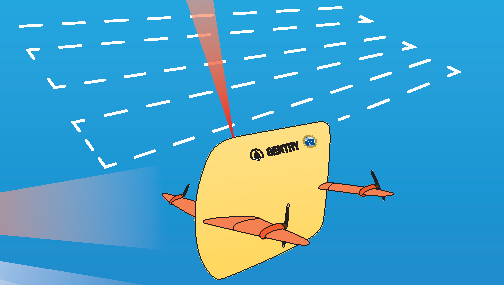
\includegraphics[width=\textwidth]{./pres/images/justSentry}
        \end{center}
      \end{figure}
%    \end{center}
  \column{.60\textwidth}

   \begin{itemize}
\item<1>Standard Model for Underwater Vehicle Dynamics
\item<1> 3-DOF Rotational Dynamics Adaptive Identification (AID) Stability Analysis
\item<1-2>    \alert<2>{6-DOF UV AID Algorithm} 
\item<1,3> \alert<3>{Experimental Evaluation: 6-DOF UV AID}
   \end{itemize}
\end{columns}
\end{frame}

%\subsection{UV Adaptive Identification}

\begin{frame}{UV Adaptive Identification}

  Plant:
  \vspace*{-5mm}

  \begin{equation*}
    \dot{v}=M^{-1}\left(\ad_{v(t)}^T(M v)+\sum_{i=1}^6 |v_i|D_i
    v+\mathcal{G}(g,b,H)+u\right)
  \end{equation*}
  \vspace*{-5mm}

  Adaptive Identifier:

  \vspace*{-5mm}

  \begin{equation*}
    \dot{\hat{v}}=\hat{M}^{-1}\left( \ad_v^T\hat{M}v
    +\sum_{i=1}^6 |v_i|\hat{D}_i v+\mathcal{G}(\hat{g},\hat{b},H)
    + u\right)- a \Delta v  
  \end{equation*}

  Parameter Update Laws:


  \begin{equation*}
    \dot{\hat{M}}=-\frac{\gamma_1}{2}\left(\psi_1 v^T 
    +v \psi_1^T-\Delta v \psi_2^T-\psi_2 \Delta v^T\right) 
  \end{equation*}

  \vspace*{-5mm}

  \begin{columns}

    \column{.33\textwidth}

    \begin{equation*}
      \dot{\hat{D_i}}=-\gamma_2|v_i|\Delta v v^T
    \end{equation*}

    \column{.33\textwidth}

    \begin{equation*}
      \dot{\hat{g}}=-\gamma_3\Delta \omega^T R^T e_3
    \end{equation*}

    \column{.33\textwidth}

    \begin{equation*}
      \dot{\hat{b}}=-\gamma_4\mathcal{J}(R^T e_3)\Delta \omega
    \end{equation*}

  \end{columns} 

  \vspace*{5mm}

  
  \alert<2->{For the technical conditions stated in the thesis, I show
    the identifier's velocity converges to the plant's velocity and
    parameter estimates converge to values that provide input-output
    behavior identical to that of the true plant for the given input
    $u(t)$.}

\end{frame}

%\begin{frame}{Implementation of Identification Algorithms}
%
%\end{frame}


\subsection{Experimental Evaluation: UV AID}

%\subsection{Experimental Overview}
\begin{frame}{Experimental Facility}

  \begin{columns}
    \column{.5\textwidth}

    Facility:
    \begin{itemize}
    \item Indoor freshwater tank (7.75 m diameter and 4.25 m deep)
    \item long baseline array - provides vehicle position
    \end{itemize}
    Johns Hopkins University Remotely Operated Vehicle (JHU ROV): 
    \begin{itemize}
    \item 150 kg vehicle 
    \item six 1.5 kWh DC brushless thrusters
    \item full 6 DOF control authority
    \item State-of-the-art sensor package
    \end{itemize}

    \column{.5\textwidth}

    \begin{center}
      \begin{figure}[htbp]  
        \begin{center}
          
\includegraphics[width=60mm]{./appenJHUHTF/images/jhurov}
        \end{center}
        \caption{JHU ROV inside the Johns Hopkins Hydrodynamic Test
          Facility.}
      \end{figure}
    \end{center}    
  \end{columns} 
\end{frame}

%\begin{frame}
%video slide!
%\end{frame}




% \begin{frame}{Experimental Cross-Validation Method}

%     \begin{itemize}
%     \item Main idea is we performed two experiments: 
%       \begin{itemize}
%       \item First Experiment used to identify plant model (\alert<2->{IDDAT})
%       \item Second Experiment used to test identified model (\alert<2->{CROSS})
%       \end{itemize}
%     \item<3-> the input signals $u^{ID}$ and $u^{CROSS}$ were different 
%     \item<4-> In both, 3 sinusoidal moments and 3 sinusoidal force inputs 
%       were simultaneously driving the vehicle
%     \end{itemize}

%   %\begin{columns}
%   %   \column{.5\textwidth}
%   %   \begin{center}
%   %     \begin{figure}[htbp]  
%   %       \begin{center}
%   %         \includegraphics[width=50mm]{./pres/images/ID_inputSketch}
%   %       \end{center}
%   %       \caption{Identification Input}
%   %     \end{figure}
%   %   \end{center}    

%   %   \column{.5\textwidth}

%   %   \begin{center}
%   %     \begin{figure}[htbp]  
%   %       \begin{center}
%   %         \includegraphics[width=50mm]{./pres/images/CROSS_inputSketch}
%   %       \end{center}
%   %       \caption{Cross-Validation  Input}
%   %     \end{figure}
%   %   \end{center}    
%   % \end{columns} 

% \end{frame}


% \begin{frame}{Identification Algorithm Evaluation Methodology}

%   \begin{columns}
%     \column{.57\textwidth}

%     \alt<1-3> { 

%       Our goal: Evaluate if the parameter estimates of adaptive
%       identification are 'good'.

%       \pause \vskip10pt
   
%       The Straightforward Approach: Compare the parameter estimates
%       of adaptive identification to those
%       \alert<2-3>{\alt<1-2>{computed analytically}{estimated with least squares}}.

%      \vskip10pt

%      Unfortunately \alert<2-3>{\alt<1-2>{$M$, $D_1$, $D_2$, $D_3$,
%      $D_4$, $D_5$, $D_6$, $g$ and $b$ cannot be computed analytically}{
%      there is no way to guarantee that parameter sets must be 'close' to
%      one another for both to accurately model vehicle dynamics}}

%     } {

%       \alert<4-5>{Better Goal}: Evaluate if parameter estimates of
%       adaptive identification and least squares identification
%       \alert<5>{provide similar capacity to model vehicle dynamics}.

%       \vskip10pt

%       \begin{itemize}
%       \item<5-> One Experiment for identification
%       \item<6-> One Experiment for cross-validation 
%       \item<7-> Estimated model used as an Open-Loop-Observer
%       \item<8-> Plant open-loop-stable in pitch, roll, and velocity
%       \item<9-> For these DOF, use Mean Absolute Error (MAE) listed metric
%         for modeling accuracy
%       \end{itemize} 
      
%     }    
    
%     \column{.43\textwidth}
%     \only<5->{
%       \begin{center}
%         \begin{figure}[htbp]  
%           \begin{center}
%             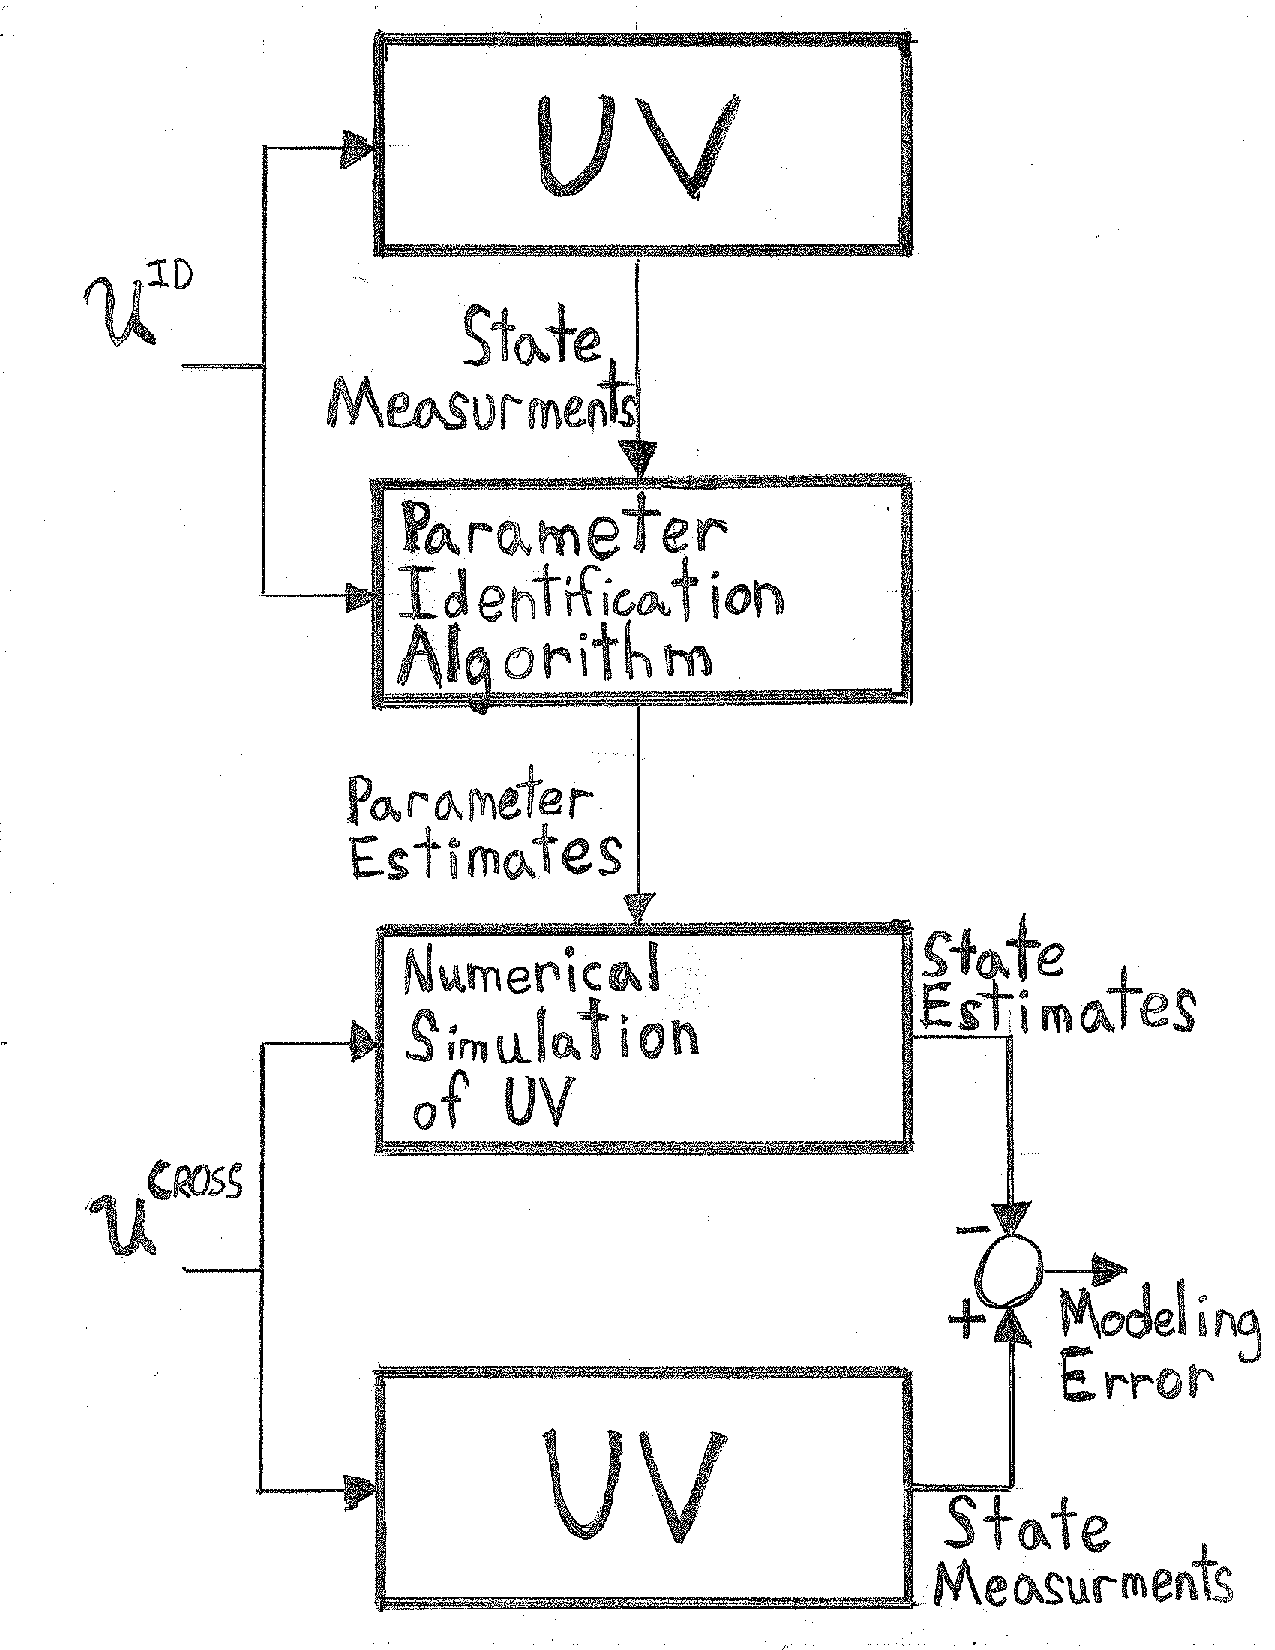
\includegraphics[width=50mm]{./pres/images/blockDiaSketch}
%           \end{center}
%         \end{figure}
%       \end{center}    

%     }  
%   \end{columns} 

% \end{frame}


\begin{frame}{Identification Algorithm Evaluation Methodology}

\begin{columns}
\column{.57\textwidth}
      \alert<1-2>{Our Goal}: Evaluate if parameter estimates of
      adaptive identification and least squares identification
      \alert<2>{provide similar capacity to model vehicle dynamics}.

      \vskip10pt

      \begin{itemize}
      \item<3-> Run two experiments 
       \begin{itemize}
       \item<3-> First experiment for parameter identification
       \item<3-> Second experiment for parameter evaluation
       \end{itemize}
     %\item<4-> Evaluation process used for \alert<6->{both Least
     %    Squares and Adaptive Identification}
     \item<3-> Compare state measurements from second experiment 
               to state estimates from UV forward simulation
      \item<3-> Mean Absolute Error (MAE) between measured and
        simulated vehicle states used to judge modeling accuracy

      \end{itemize} 
    
    \column{.43\textwidth}
     \only<3->{
      \begin{center}
        \begin{figure}[htbp]  
          \begin{center}
            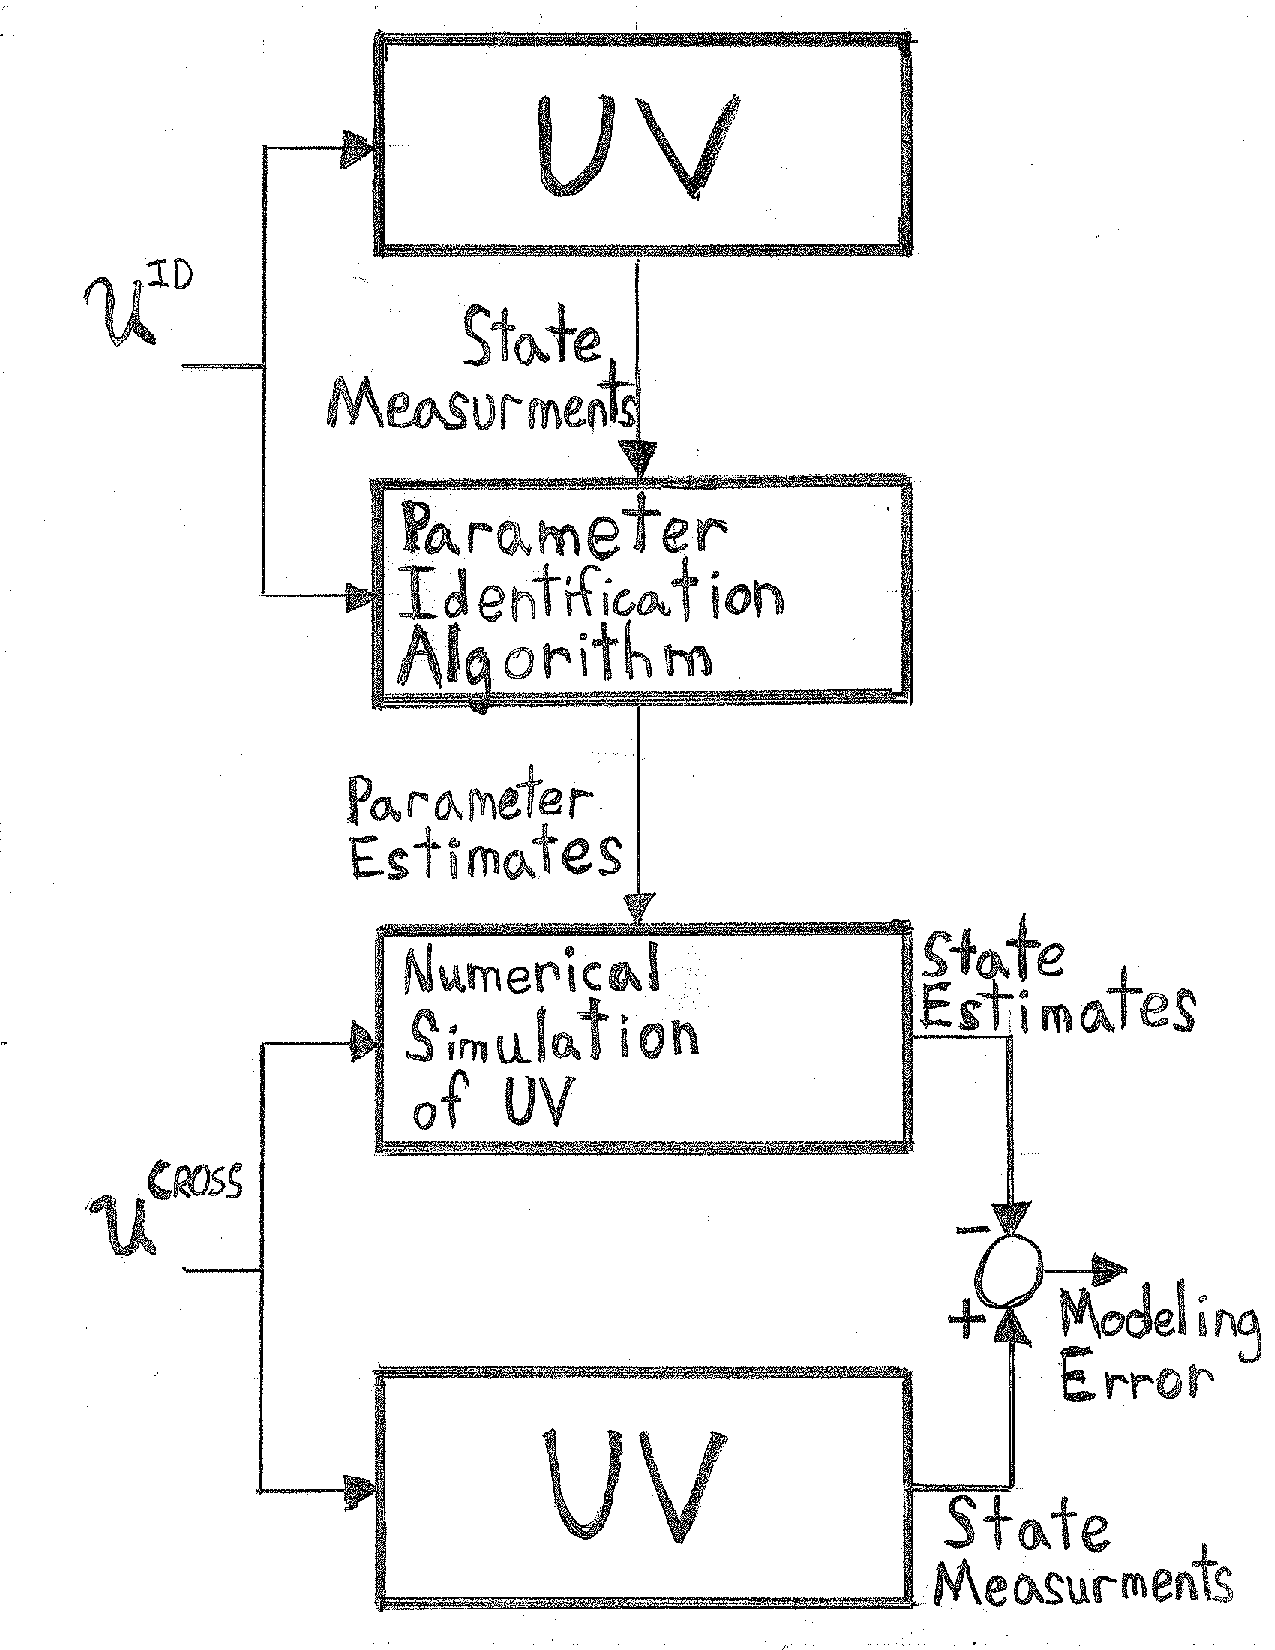
\includegraphics[width=50mm]{./pres/images/blockDiaSketch}
          \end{center}
        \end{figure}
      \end{center}    
      }
  \end{columns} 

\end{frame}

%\subsection{Cross-Validation Experiment}

\begin{frame}{Angular Position Sample Data: Roll Degree-of-Freedom}
    
    \begin{center}
      \begin{figure}[htbp]
        \begin{center}
          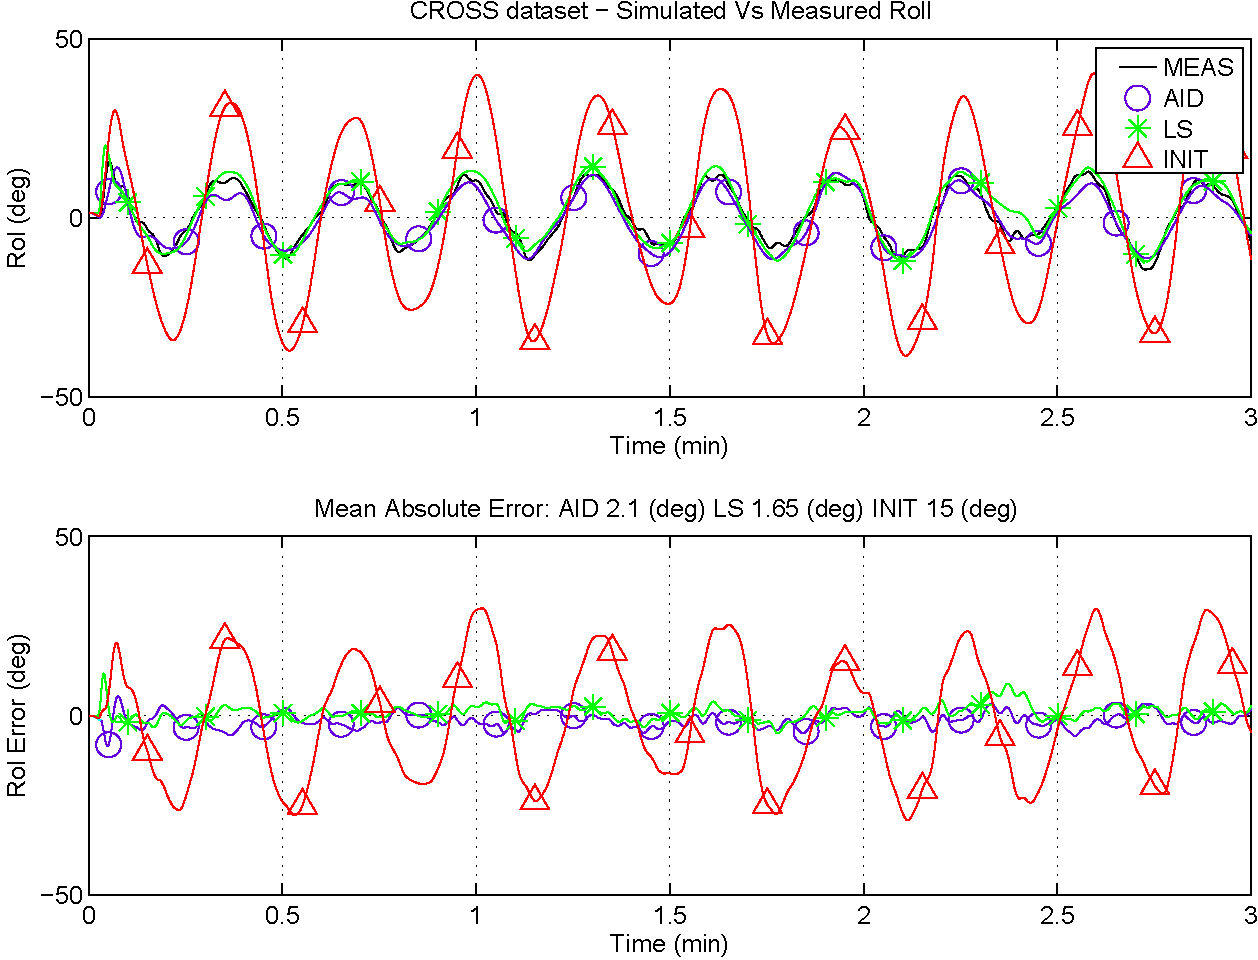
\includegraphics[width=3.5in]{./pres/images/crossALL_posExDOF_2}
        \end{center}
      \end{figure}
    \end{center}
   
\end{frame}

\begin{frame}{Analysis: Cross-Validation Experiment}

%{ \scriptsize
%\begin{table}[htbp]
%\caption{Mean Absolute Error Values for Cross-Validation Experiment}
%\begin{center}
%\begin{tabular}{p{1.5cm}|cccccccc}
% & \multicolumn{2}{c}{Angular Pose} & \multicolumn{3}{c}{Translational Velocity}& \multicolumn{3}{c}{Angular Velocity} \\ 
%Parameter Set & Roll & Pitch & x DOF & y DOF & z DOF & x DOF & y DOF & z DOF \\ \hline
%AID  &  2.0$^\circ$ & 2.1$^\circ$ & 0.062 m/s & 0.058 m/s & 0.037 m/s & 1.39$^\circ$/s & 1.35$^\circ$/s & 5.0$^\circ$/s \\
%LS   &  1.38$^\circ$ & 1.65$^\circ$ & 0.050 m/s & 0.052 m/s & 0.024 m/s & 1.38$^\circ$/s & 1.39$^\circ$/s & 6.3$^\circ$/s \\
%INIT & 9.9$^\circ$ & 15.0$^\circ$ & 0.165 m/s & 0.26 m/s & 0.25 m/s & 5.1$^\circ$/s & 3.3$^\circ$/s & 3.9$^\circ$/s \\
%\end{tabular}
%\end{center}
%\end{table}
%}
{ \scriptsize
\begin{table}[htbp]
\caption{Mean Absolute Error Values for Cross-Validation Experiment}
\begin{center}
\begin{tabular}{p{1.5cm}|cccccccc}
 & \multicolumn{2}{c}{Angular Pose ($^\circ$)} & \multicolumn{3}{c}{Translational Velocity (m/s) }& \multicolumn{3}{c}{Angular Velocity ($^\circ$/s)} \\ 
Parameter Set & Roll & Pitch & x DOF & y DOF & z DOF & x DOF & y DOF & z DOF \\ \hline
AID  &  2.0 & 2.1 & 0.062  & 0.058  & 0.037  & 1.39 & 1.35 & 5.0 \\
LS   &  1.38 & 1.65 & 0.050  & 0.052 & 0.024  & 1.38 & 1.39 & 6.3 \\
INIT & 9.9 & 15.0 & 0.165  & 0.26  & 0.25 & 5.1 & 3.3 & 3.9 \\
\end{tabular}
\end{center}
\end{table}
}
 \begin{itemize}
   \item<2-> Experimentally identified parameters model vehicle's action better 
   \item<3-> Similar modeling error by AID and LS
   \item<4-> LS might be marginally better at matching angular position
%  \item<5->
%    Adaptive Identification does not require vehicle acceleration to be instrumented
 \end{itemize}

\end{frame}


  

%\begin{frame}{Angular Velocity Sample Data: Degree-of-Freedom Y}
%    \begin{center}
%      \begin{figure}[htbp]
%        \begin{center}
%          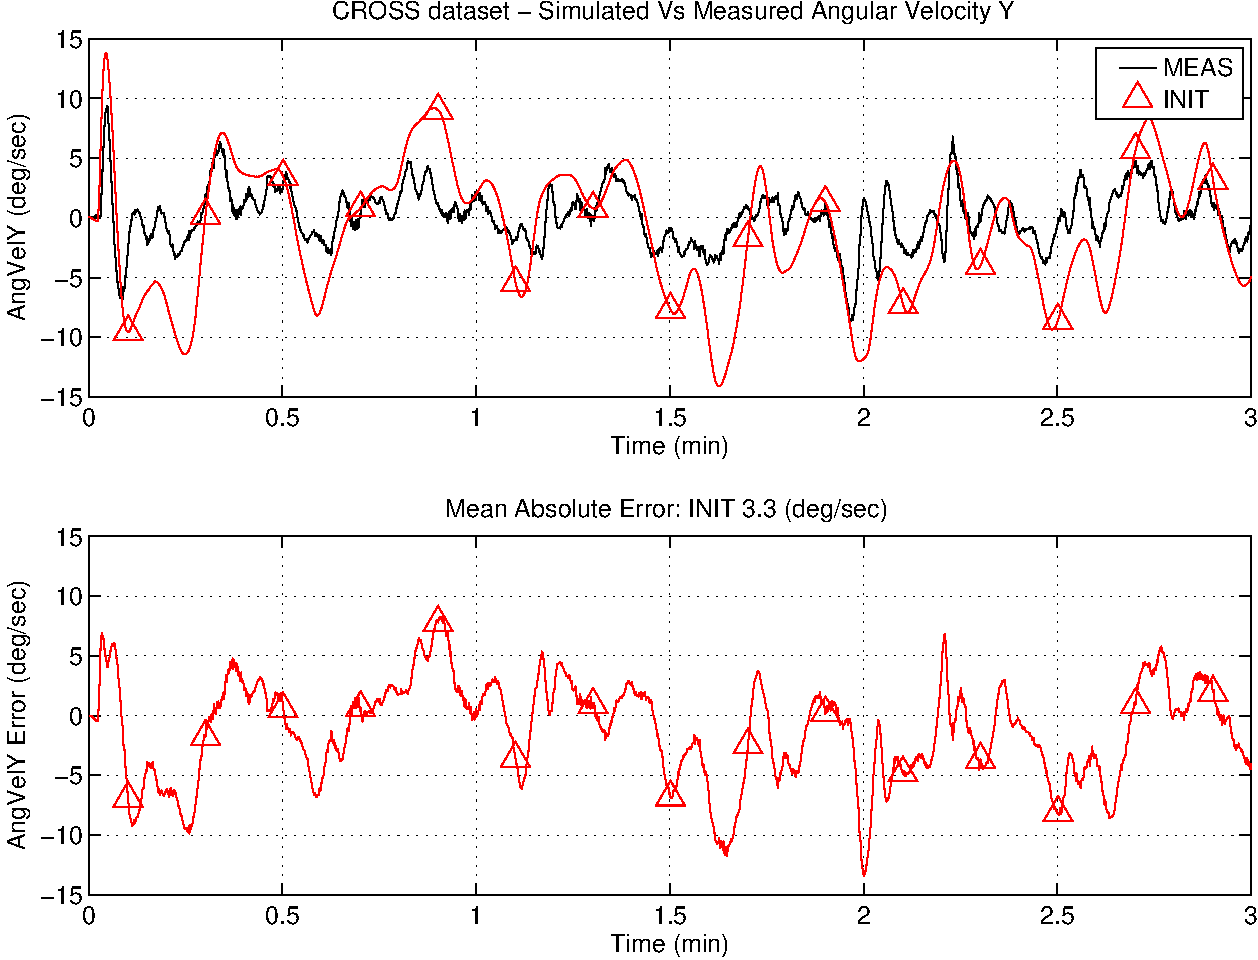
\includegraphics[width=3.75in]{./pres/images/crossINIT_angVelExDOF}
%        \end{center}
%      \end{figure}
%    \end{center}
%    
%\end{frame}  
  
\begin{frame}{Angular Velocity Sample Data: Degree-of-Freedom Y}
    
    \begin{center}
      \begin{figure}[htbp]
        \begin{center}
          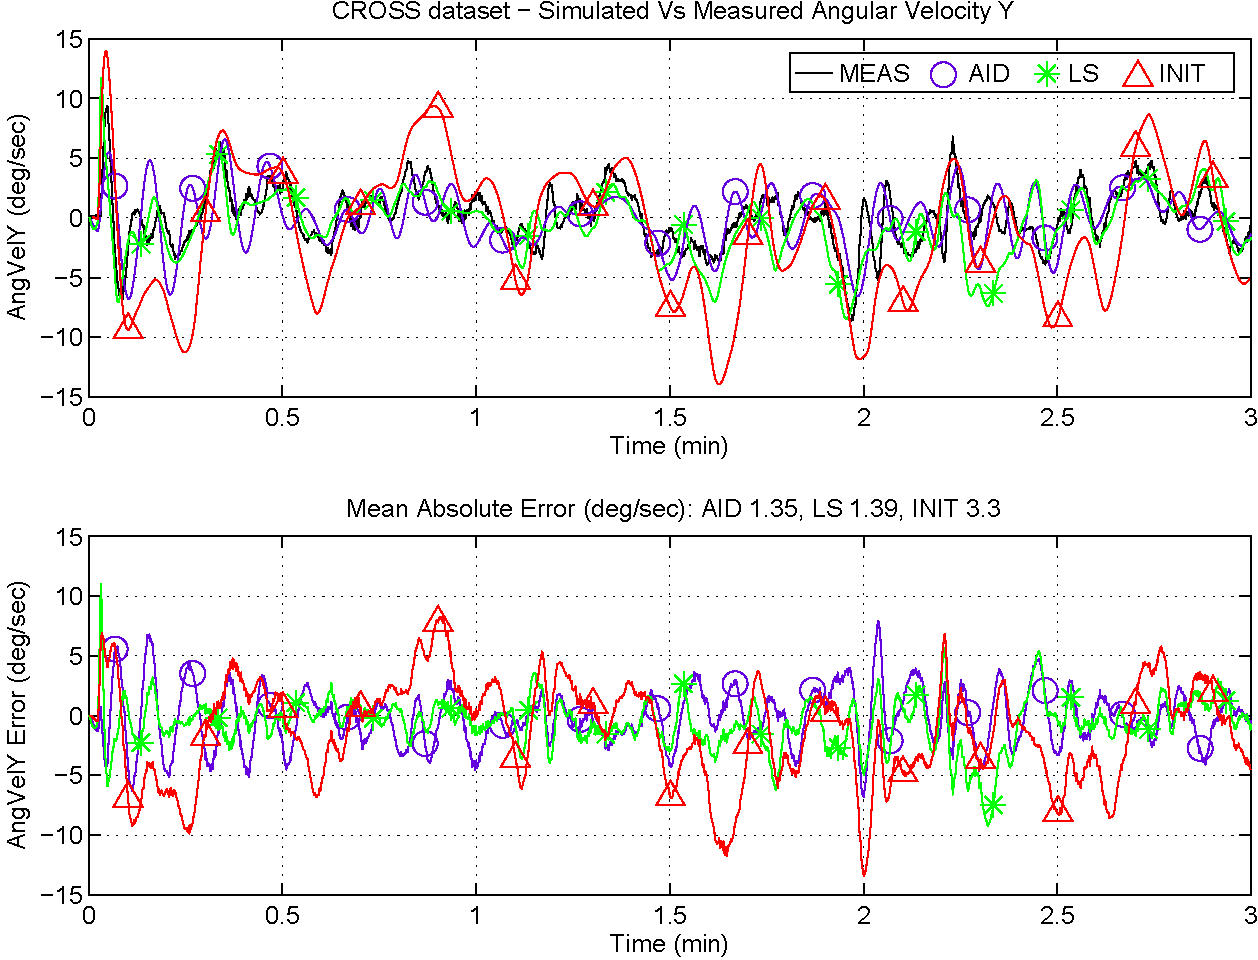
\includegraphics[width=3.75in]{./pres/images/crossAID_angVelExDOF_all}
        \end{center}
      \end{figure}
    \end{center}
   
\end{frame}


%\begin{frame}{Body Velocity Sample Data: Degree-of-Freedom Z}
%    \begin{center}
%      \begin{figure}[htbp]
%        \begin{center}
%          \includegraphics[width=3.75in]{./pres/images/crossINIT_transVelExDOF}
%        \end{center}
%      \end{figure}
%    \end{center}
    
%\end{frame}  
  
%\begin{frame}{Body Velocity Sample Data: Degree-of-Freedom Z}
%    
%    \begin{center}
%      \begin{figure}[htbp]
%        \begin{center}
%          \includegraphics[width=3.75in]{./pres/images/crossAID_transVelExDOF}
%        \end{center}
%      \end{figure}
%    \end{center}
%   
%\end{frame}


\begin{frame}{Adaptive Identification Summary}

  % Keep the summary *very short*.

   \begin{columns}
      \column{.40\textwidth}
 %   \begin{center}
      \begin{figure}[t!]
        \begin{center}
          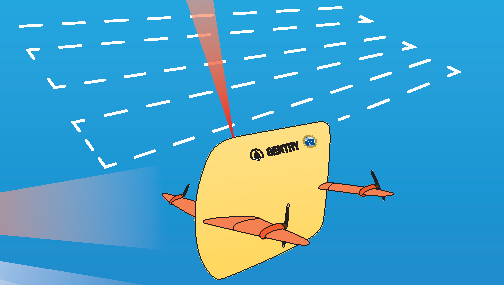
\includegraphics[width=\textwidth]{./pres/images/justSentry}
        \end{center}
      \end{figure}
%    \end{center}
  \column{.60\textwidth}
 \begin{itemize}
  \item
    Adaptive Identification provided a good model of UV Dynamics.
  \item Least Squares and Adaptive Identification provided a similar
    capacity to model UV.
  \item Adaptive identification algorithms do not require simultaneous
    reference trajectory-tracking control, nor do they require
    instrumentation of linear acceleration or angular acceleration;
  \item Together, these facts make adaptive identification applicable
    to a wider class of UVs than previously reported methods.
  \end{itemize}
\end{columns}


  
% \pause
%  % The following outlook is optional.
%  \vskip0pt plus.5fill
%  \begin{itemize}
%  \item
%    Outlook
%    \begin{itemize}
%    \item
%      Adaptive Tracking Control for fully coupled UUV models
%    \item
%      Future directions: state observers, Coupled Adaptive Identification/Control for Fault Detection and recovery
%    \end{itemize}

\end{frame}


\section{UV Adaptive Model-Based Control}


\begin{frame}{Outline}

  \tableofcontents
  % You might wish to add the option [pausesections]

\end{frame}


\begin{frame}[t]{Adaptive Model-Based Control, Overview}%{LS Model Identification}
   \begin{columns}
      \column{.40\textwidth}
    \begin{center}
      \begin{figure}[htbp]
        \begin{center}
          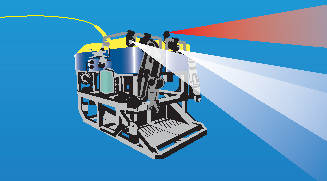
\includegraphics[width=\textwidth]{./pres/images/justJason}
        \end{center}
      \end{figure}
    \end{center}
  \column{.6\textwidth}

   \begin{itemize}
\item \alert<5>{ 6-DOF UV Model-Based Control (MBC)}
\item<1-4> 6-DOF UV Adaptive Model-Based Control (AMBC)
\item<1-4> Experimental Analysis: Thruster Dynamics and AMBC
\item<1-4> Experimental Evaluation: UV Two-Step AMBC
   \end{itemize}
\end{columns}
\vskip9pt
\uncover<1-4>{
\pause
Previous Research into UV Adaptive Model-Based Control (AMBC):
\pause
\begin{itemize}
\item Previous AMBC algorithms have been reported
\begin{itemize}
\item We report a novel AMBC algorithm which uses geometric control
  techniques to develop an error system which evolves on SE(3)
\end{itemize}
\pause
\item Previous AMBC experimental evaluations have been reported, but
  none have considered
\begin{itemize}
\item simultaneous motion in all DOF and
\item destabilizing effects of unmodeled thruster dynamics.
\end{itemize}
\end{itemize}}
\end{frame}

\subsection{UV Model-Based Control and Adaptive Extension}
\begin{frame}{UV {\it Non-Adaptive} Model-Based Control (MBC): Goal and State Representations}

\begin{columns}
      
  \column{.57\textwidth} MBC Goal: Design a control law ,
  {\color{green} $u$}, which uses the {\color{cyan} current vehicle
    state}, {\color{blue} a desired trajectory}, and {\color{red}
    known vehicle model} to provide asymptotically exact trajectory
  tracking.

      \begin{itemize}
      \item<2-> {\it actual} vehicle position {\color{cyan} ${^w_a}H$
        } and velocity {\color{cyan} ${^a}v_a$}
      \item<3-> {\it desired} vehicle position {\color{blue}
          ${^w_d}H$}, velocity {\color{blue} ${^d}v_d$}, and
        acceleration {\color{blue} ${^d}\dot{v}_d$}
      \item<4-> The vehicle parameters ${\color{red} M},~{\color{red}
          D},~{\color{red} g},~\text{and}~{\color{red} b}$ {\it are
          known}.  We will represent them using the parameter vector
        ${\color{red} \theta_{UV}}\in\rSp{241}$.
      \end{itemize} 

% \vspace*{10mm}
% \alt<1-4>{ 


% %      \vskip10pt
% }
% {

% }
    \column{.43\textwidth}
\uncover<5->{Error Coordinates}
\begin{itemize}
\item<5-6> \uncover<1-5>{$\Delta H={^w_d}H^{-1}{^w_a}H$} 
\begin{itemize}
\item<5-6> \alert<6>{$\Delta \psi=\log_{\SE3}\left(\Delta H \right)$}
\end{itemize}
\item<5-6> \alert<6>{$\Delta v={^a}v_a-{^a}v_d$}
\item<5> $\Delta \dot{H}=\Delta H\widehat{\Delta v}$
\begin{itemize}
\item $\Delta \dot{ \psi} = \hat{\mathcal{A}}^{-1}(\Delta \psi) \Delta v$
\end{itemize}
\item<5> $\Delta\dot{ v} = {^a}\dot{v}{_a}-{^a}\dot{v}{_d}+\ad_{\Delta v} {^a}v_d$
\item<5> $\hat{\mathcal{A}}^{-1}$ is the inverse of the se(3) velocity  
\end{itemize}


     \only<5->{
      \begin{center}
        \begin{figure}[htbp]  
          \begin{center}
  %          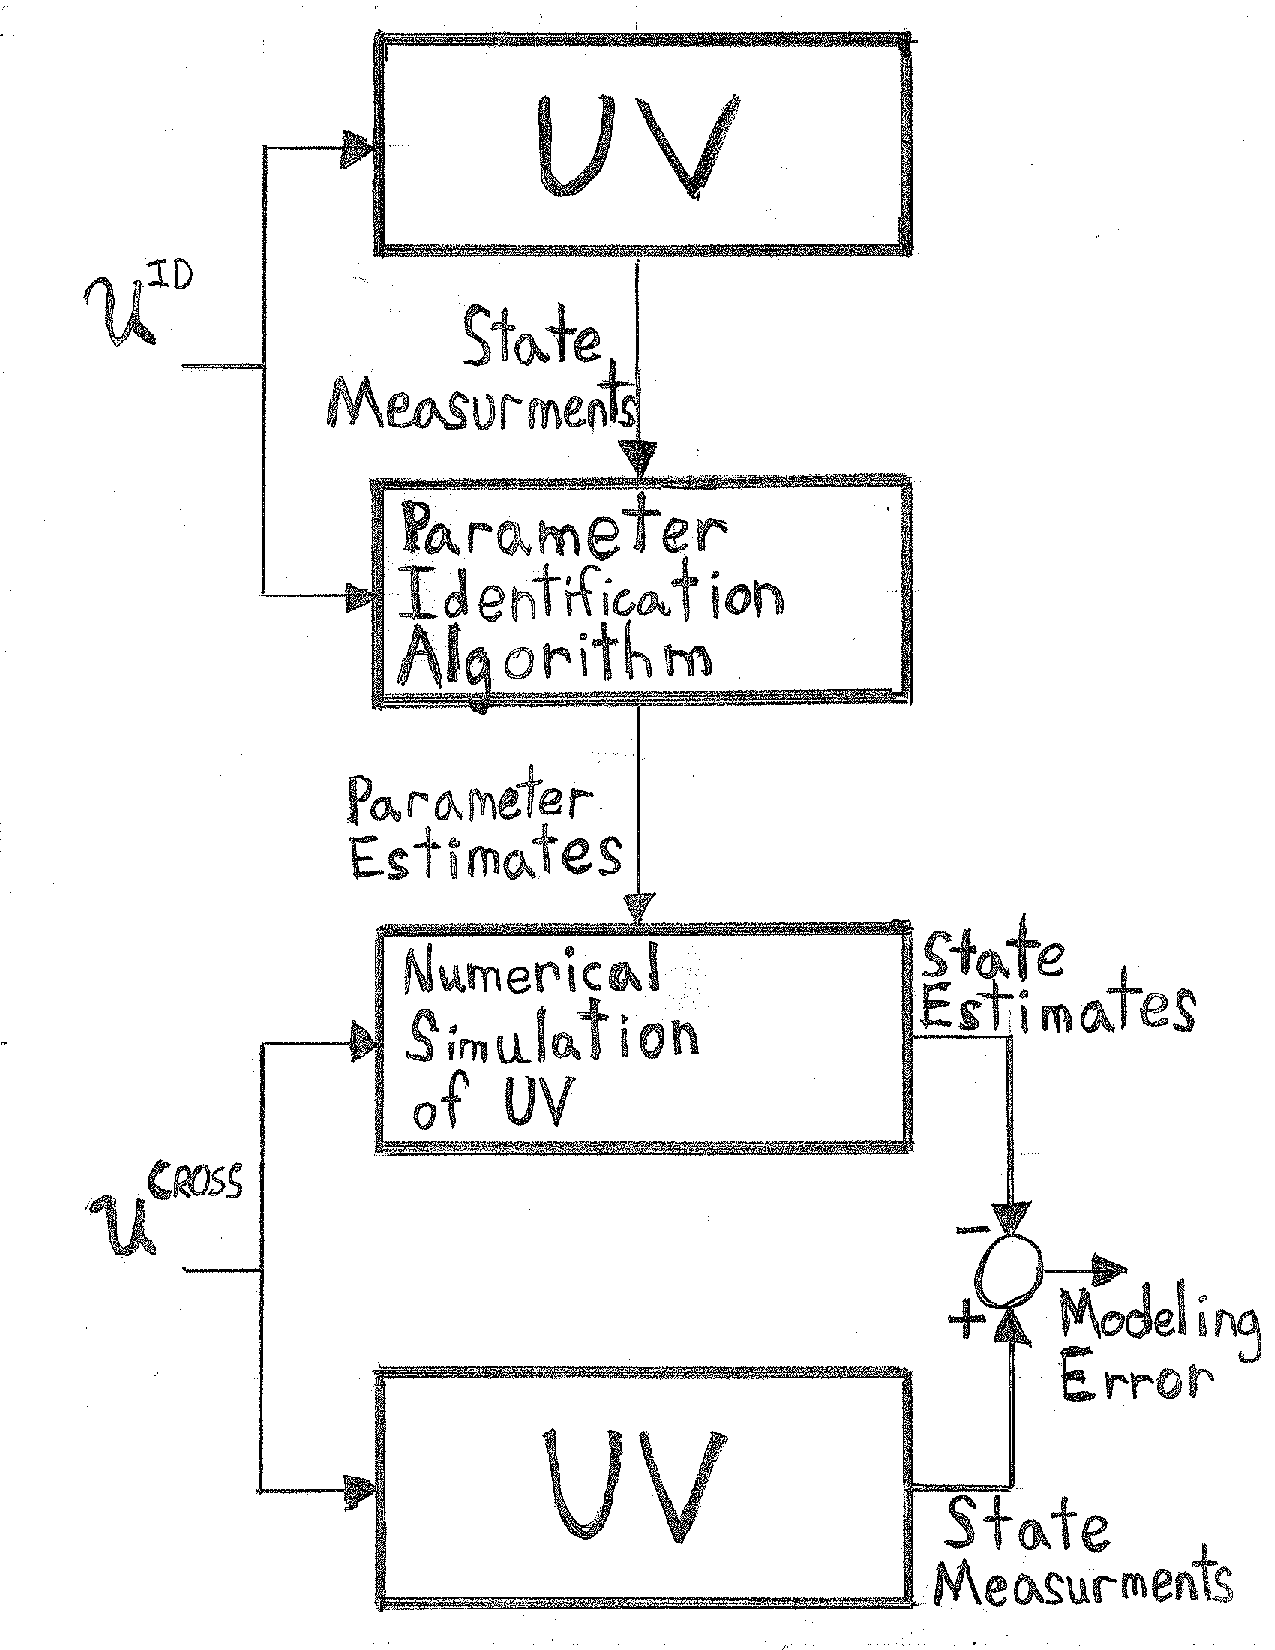
\includegraphics[width=50mm]{./pres/images/blockDiaSketch}
          \end{center}
        \end{figure}
      \end{center}    
      }
  \end{columns} 

\end{frame}



\begin{frame}[t]{Underwater Vehicle (non-adaptive) Model-Based Control}%{LS Model Identification}

%     \begin{columns}
%        \column{.3\textwidth}
% Plant Model:
%  \vskip10pt
% Control Law:
%  \vskip10pt
% Regressor:
%  \vskip10pt
%        \column{.7\textwidth}
%  \begin{align} 
%    \dot{H}(t)&={\color{cyan}H(t)}\widehat{{\color{cyan} v(t)}}
%    \nonumber \\
%    \alert{M}\dot{v}(t)&=\mathcal{H}(\alert{M}{\color{cyan} v(t)} ) {\color{cyan} v(t)}+
%    \sum_{i=1}^6 |{\color{cyan}v_i} |\alert{D_i}
%             {\color{cyan}v(t)}+
%    \mathcal{G}(\alert{g},\alert{b},{\color{cyan}H(t)})+\color{green}u(t)
%    \nonumber 
% \end{align}
% %
% \begin{equation*}
% u\left( {^w_a}H, {^a}v_a, {^w_d}H, {^d}v_d, {^d}\dot{v}_d\right)
% =-(k_p\hat{\mathcal{A}}^{-T}(\Delta \psi)+k_d\Delta v)+ 
% \MBCreg({^a}\dot{v}_d,\Delta v, {^a}v_d , {^w_a}H)\theta_{UV}
% \end{equation*}
% %
% \begin{equation*}
% \MBCreg({^a}\dot{v}_d,\Delta v, {^a}v_d , {^w_a}H)\theta_{UV} =
%     M{^a}\dot{v}_d - M\ad_{\Delta v}{^a}v_d -\ad_{{^a}v_a}^T M{^a}v_a
%     -\mathcal{D}({^a}v_a)-\mathcal{G}({^w_a}H)
% \end{equation*}
% \end{columns}


% {\small
% \begin{align} 
% \text{Plant Model:}\quad&\begin{cases}\dot{H}(t)&={\color{cyan}H(t)}\widehat{{\color{cyan} v(t)}}
%    \\
%    \alert{M}\dot{v}(t)&=\mathcal{H}(\alert{M}{\color{cyan} v(t)} ) {\color{cyan} v(t)}+
%    \sum_{i=1}^6 |{\color{cyan}v_i} |\alert{D_i}
%             {\color{cyan}v(t)}+
%    \mathcal{G}(\alert{g},\alert{b},{\color{cyan}H(t)})+\color{green}u(t)
%    \end{cases}
% \nonumber \\
% \text{Control Law:}\quad&u\left( {^w_a}H, {^a}v_a, {^w_d}H, {^d}v_d, {^d}\dot{v}_d\right)
% =-(k_p\hat{\mathcal{A}}^{-T}(\Delta \psi)+k_d\Delta v)+ 
% \MBCreg({^a}\dot{v}_d,\Delta v, {^a}v_d , {^w_a}H)\theta_{UV}
% \nonumber \\
% \text{Regressor:}\quad&\MBCreg({^a}\dot{v}_d,\Delta v, {^a}v_d , {^w_a}H)\theta_{UV} =
%     M{^a}\dot{v}_d - M\ad_{\Delta v}{^a}v_d -\ad_{{^a}v_a}^T M{^a}v_a
%     -\mathcal{D}({^a}v_a)-\mathcal{G}({^w_a}H)
% \nonumber 
% \end{align}
% }



{\small
\begin{align} 
\text{Plant Model:}\quad&\begin{cases}{^w_a}\dot{H}&={\color{cyan}{^w_a}H}\widehat{{\color{cyan} {^a}v_a}}
   \\
   \alert{M}{^a}\dot{v}_a&=\ad_{\color{cyan} {^a}v_a}^T\alert{M}{\color{cyan} {^a}v_a} +
   \sum_{i=1}^6 |{\color{cyan}{^a}v_{ai}} |\alert{D_i}
            {\color{cyan}{^a}v_a}+
   \mathcal{G}({\color{cyan}{^w_a}H})+\color{green}u
   \end{cases}
\nonumber \\
\text{Control Law:}\quad&u%\left( {^w_a}H, {^a}v_a, {^w_d}H, {^d}v_d, {^d}\dot{v}_d\right)
=-k_p\hat{\mathcal{A}}^{-T}(\Delta \psi)-k_d\Delta v+ 
\MBCreg\theta_{UV}
\nonumber \\
\MBCreg~ \text{such that:}\quad&\MBCreg\theta_{UV} =
    M{^a}\dot{v}_d - M\ad_{\Delta v}{^a}v_d -\ad_{{^a}v_a}^T M{^a}v_a
    -\sum_{i=1}^6 |{{^a}v_{ai}} |D_i
            {{^a}v_a}-\mathcal{G}({^w_a}H)
\nonumber 
\end{align}
\vskip7pt
\vskip7pt
\pause
This control law provides locally asymptotically stable trajectory tracking in the
sense of Lyapunov, i.e.  $\lim_{t\to \infty}\Delta \psi(t)=\vec{0}$
and $\lim_{t\to \infty}\Delta v(t)=\vec{0}$, if the following
conditions are met:

\begin{itemize}
\item the signals $\{{^w_d}H,{^d}v_d,{^d}\dot{v}_d
  \}\in\{\SE3,\realSpace{6},\realSpace{6}\}$ are continuous and bounded
\item $k_d,k_p\in\mathbb{R}_+$
\item $\|x(t_0)\|<\sqrt{
                  \frac{ {_\epsilon}\lambda_{12} }
                       { {_\epsilon}\lambda_1   }
                       } \pi$ 
\end{itemize}

\noindent where ${_\epsilon}\lambda_{1}$ and ${_\epsilon}\lambda_{12}$
are the largest and smallest eigenvalues, respectively, of
$\mathcal{M}_\epsilon\in\rSp{12\times 12}$ from the Lyapunov function.}


\end{frame}


\begin{frame}[t]{Outline of MBC Stability Analysis}
\begin{align}
\text{Error Dynamics:}\quad &\left[ \begin{array}{c}
     \Delta \dot{\psi}           \\
     \Delta \dot{v}              \\
\end{array} \right]=
\left[ \begin{array}{cc}
     0_{6\times 6}   & \hat{\mathcal{A}}^{-1}(\Delta \psi)             \\
     -k_p M^{-1}\hat{\mathcal{A}}^{-T}(\Delta \psi)   &  -k_d M^{-1}   \\
\end{array} \right]\left[ \begin{array}{c}
     \Delta \psi           \\
     \Delta v              \\
\end{array} \right]
\nonumber \\
\text{Lyapunov Fn:}\quad & 
V_1(t)=\frac{1}{2} \left[\begin{array}{cc}
   \Delta \psi^T & \Delta v^T
   \end{array} \right]
\left[ 
\begin{array}{cc}
  k_p\mathbb{I}_{6\times 6}  & \epsilon M         \\
  \epsilon M               &    M               \\
\end{array} \right]\left[ \begin{array}{c}
     \Delta \psi           \\
     \Delta v              \\
\end{array} \right]
\nonumber \\
\text{Lyap Derivative:}\quad & \dot{V}_1(t) \leq\frac{1}{2}\left[\begin{array}{cc}
   \|\Delta \psi\| & \|\Delta v\|
   \end{array} \right] 
  \left[\begin{array}{cc}
  -\epsilon 2 k_p  & \epsilon k_d    \\
 \epsilon k_d      &   \epsilon \lambda_1 c- 2k_d\\
  \end{array} \right] 
\left[\begin{array}{c}
   \|\Delta \psi\| \\ \|\Delta v\|
\end{array} \right] 
\nonumber
\end{align}

\pause

\begin{itemize}
\item For all $\epsilon\in\rSp{}_+$ such that
  $\epsilon\leq\min\left(\frac{4 k_p k_d}{2 \lambda_1 k_p c
      +k_d^2},\sqrt{\frac{k_p \lambda_6}{\lambda_1^{2}}} \right)$
  \\local asymptotically exact trajectory-tracking is proven
\item Several Properties for $\hat{\mathcal{A}}^{-1}(\Delta \psi)$
  required:
\begin{itemize}
\item $c$ is bound of $\|\hat{\mathcal{A}}^{-1}(\Delta \psi)\|$, local
  result required for bounded $c$
\item $\Delta\psi^T\left(\hat{\mathcal{A}}^{-T}+\hat{\mathcal{A}}^{-1}\right)\Delta
\psi=\Delta\psi^T\Delta\psi$
\end{itemize}
\item Facts proven in Appendices
\end{itemize}
\end{frame}


\begin{frame}{UV {\it Adaptive} Model-Based Control (AMBC): Goal and State Representations}

 
 

   \begin{columns}
      
     \column{.57\textwidth} AMBC Goal: Design a control law,
     {\color{green} $u$}, and parameter estimate update law, {\color{red}
       $\dot{\hat{\theta}}_{UV}$}, which uses the {\color{cyan}
       current vehicle state} and {\color{blue} desired trajectory}
     provide asymptotically exact trajectory tracking for a vehicle
     while all signals remain stable assuming the plant parameters are
     constant but unknown.  % \vskip10pt


      \begin{itemize}
     \item<2-> {\it actual} vehicle position {\color{cyan} ${^w_a}H$
        } and velocity {\color{cyan} ${^a}v_a$}
      \item<3-> {\it desired} vehicle position {\color{blue}
          ${^w_d}H$}, velocity {\color{blue} ${^d}v_d$}, and
        acceleration {\color{blue} ${^d}\dot{v}_d$}
      \item<4-> The vehicle parameters ${\color{red} M},~{\color{red}
          D},~{\color{red} g},~\text{and}~{\color{red} b}$ are {\it
          unknown}: we will use the parameter estimate vector
        ${\color{red} \hat{\theta}_{UV}}\in\rSp{241}$ and parameter
        error coordinates $\Delta\theta=\hat{\theta}_{UV}-\theta_{UV}$
      \end{itemize}
%
      \vspace*{10mm}
%

%
    \column{.43\textwidth} \only<2->{
      \begin{center}
        \begin{figure}[htbp]
          \begin{center}
  % 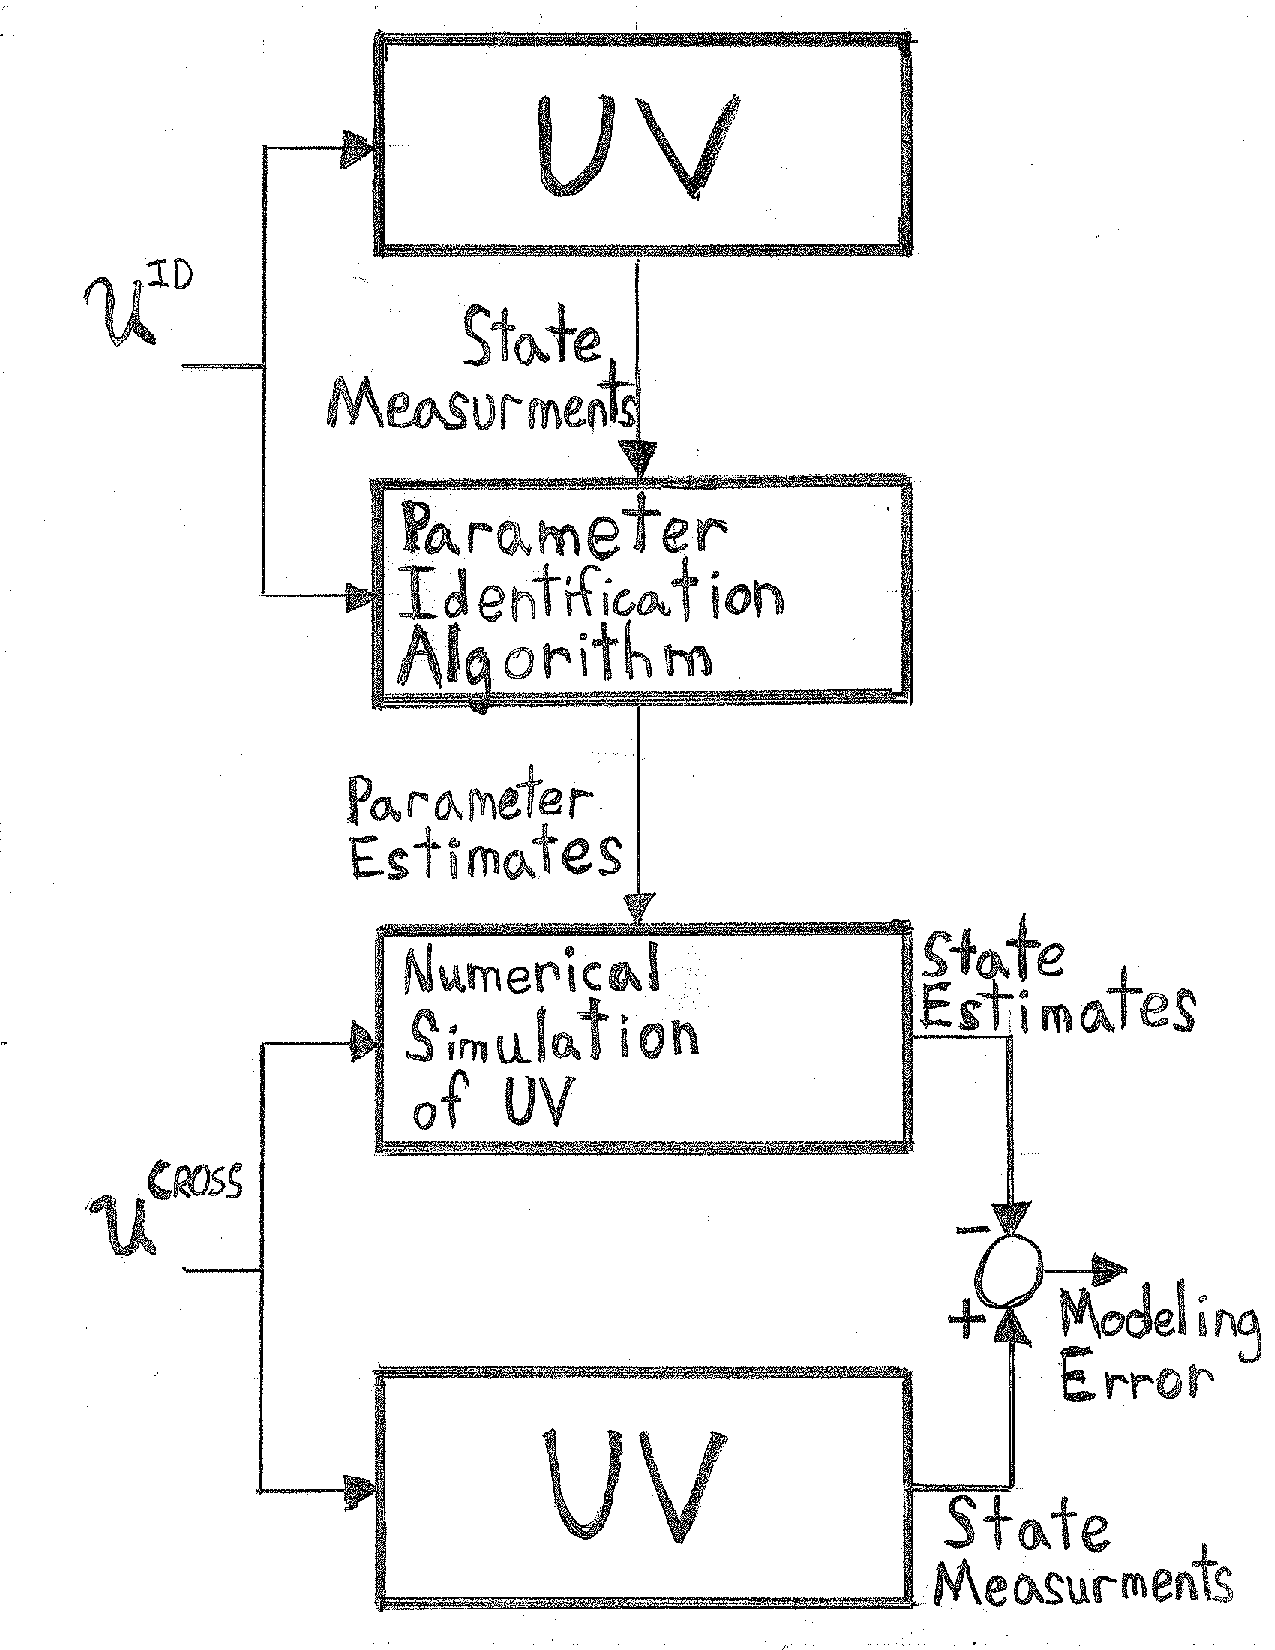
\includegraphics[width=50mm]{./pres/images/blockDiaSketch}
          \end{center}
        \end{figure}
      \end{center} }
  \end{columns}
\end{frame}



\begin{frame}[t]{Underwater Vehicle Adaptive Model-Based Control}

{\small
\begin{align} 
\text{Plant Model:}\quad&\begin{cases}\dot{H}(t)&={\color{cyan}H(t)}\widehat{{\color{cyan} v(t)}}
   \\
   \alert{M}\dot{v}(t)&=\ad_{\color{cyan} v(t)}^T\alert{M}{\color{cyan} v(t)} +
   \sum_{i=1}^6 |{\color{cyan}v_i} |\alert{D_i}
            {\color{cyan}v(t)}+
   \mathcal{G}(\alert{g},\alert{b},{\color{cyan}H(t)})+\color{green}u(t)
   \end{cases}
\nonumber \\
\text{Control Law:}\quad&u%\left( {^w_a}H, {^a}v_a, {^w_d}H, {^d}v_d, {^d}\dot{v}_d\right)
=-k_p\hat{\mathcal{A}}^{-T}(\Delta \psi)-k_d\Delta v+ 
\MBCreg\hat{\theta}_{UV}
\nonumber \\
\hat{\theta}_{UV}\text{ Update Law:}\quad&\dot{\hat{\theta}}
 =-K_\theta \MBCreg^T [\epsilon \Delta \psi +\Delta v]
\nonumber \\
\MBCreg~ \text{such that:}\quad&\MBCreg\hat{\theta}_{UV} =
    \hat{M}{^a}\dot{v}_d - \hat{M}\ad_{\Delta v}{^a}v_d -\ad_{{^a}v_a}^T \hat{M}{^a}v_a
    -\sum_{i=1}^6 |{{^a}v_{ai}} |\hat{D}_i
            {{^a}v_a}-\hat{\mathcal{G}}({^w_a}H)
\nonumber 
\end{align}


\pause This control law and parameter update law provide locally
asymptotically stable trajectory tracking and parameter estimates
which converge to constant values, i.e. $\lim_{t\to
  \infty}\dot{\hat{\theta}}(t)=0_{241 \times 1}$, if the MBC stability
conditions are met and:
%
\begin{itemize}
\item $K_\theta$ is SPD
\item $\epsilon<\min\left(\frac{4 k_p k_d}{2 \lambda_1 k_p c
    +k_d^2},\sqrt{\frac{k_p \lambda_6}{\lambda_1^{2}}} \right)$
\item $\sqrt{
      \frac{{_\epsilon}\lambda_1}{{_\epsilon}\lambda_{12}}\|x(t_0)\|^2+
      \frac{k_\theta}{{_\epsilon}\lambda_{12}}\|\Delta \theta(t_0)\|^2
       } <\pi$.
\end{itemize}
%
\noindent where $k_{\theta}=\frac{1}{\min{\eig{K_\theta}}}$ and
$\lambda_{1}$ and $\lambda_{6}$ are the largest and smallest
eigenvalues of $M$.}
\end{frame}



\begin{frame}[t]{Outline of AMBC Stability Analysis}
\begin{align}
\text{Error Dynamics:}\quad &\left[ \begin{array}{c}
     \Delta \dot{\psi}           \\
     \Delta \dot{v}              \\
\end{array} \right]=\hat{\mathbb{A}}(\Delta \psi)
\left[ \begin{array}{c}
     \Delta \psi           \\
     \Delta v              \\
\end{array} \right]+
\left[\begin{array}{c}
   0_{6\times 1}   \\ M^{-1}\MBCreg \Delta \theta
   \end{array} \right] 
\nonumber \\
\text{Lyapunov Fn:}\quad & 
V_2(t)=V_1(t)+ \frac{1}{2}\Delta\theta^T K_\theta^{-1} \Delta \theta
\nonumber \\
\text{Lyap Derivative:}\quad & \dot{V}_2(t) =\dot{V}_1(t)
%\leq\frac{1}{2}\left[\begin{array}{cc}
%   \|\Delta \psi\| & \|\Delta v\|
%   \end{array} \right] 
%  \left[\begin{array}{cc}
%  -\epsilon 2 k_p  & \epsilon k_d    \\
% \epsilon k_d      &   \epsilon \lambda_1 c- 2k_d\\
%  \end{array} \right] 
%\left[\begin{array}{c}
%   \|\Delta \psi\| \\ \|\Delta v\|
%\end{array} \right] 
\nonumber
\end{align}

\begin{itemize}
\item  Stability analysis builds off MBC stability analysis: $\hat{\mathbb{A}}(\Delta \psi)=\left[ \begin{array}{cc}
     0_{6\times 6}   & \hat{\mathcal{A}}^{-1}(\Delta \psi)             \\
     -k_p M^{-1}\hat{\mathcal{A}}^{-T}(\Delta \psi)   &  -k_d M^{-1}   \\
\end{array} \right]$
\pause
\item As with MBC, for all $\epsilon\in\rSp{}_+$ such that $\epsilon\leq\min\left(\frac{4 k_p k_d}{2 \lambda_1 k_p c
    +k_d^2},\sqrt{\frac{k_p \lambda_6}{\lambda_1^{2}}} \right)$ \\ local asymptotically exact trajectory-tracking is proven.
\item In addition to MBC conditions on initial state of the system, now conditions on the initial parameter error
      are required to maintain the bounded $c$.
\end{itemize}
\end{frame}


\subsection{Experimental Evaluation: UV AMBC}


\begin{frame}[t]{Adaptive Model-Based Control, Overview}%{LS Model Identification}
   \begin{columns}
      \column{.40\textwidth}
    \begin{center}
      \begin{figure}[htbp]
        \begin{center}
          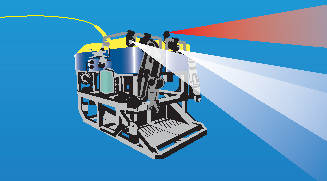
\includegraphics[width=\textwidth]{./pres/images/justJason}
        \end{center}
      \end{figure}
    \end{center}
  \column{.6\textwidth}

   \begin{itemize}
\item<1> 6-DOF UV Model-Based Control (MBC)
\item<1> 6-DOF UV Adaptive Model-Based Control (AMBC)
\item<1-2,4> Experimental Analysis: Thruster Dynamics and AMBC
\item<1,3-4> Experimental Evaluation: UV Two-Step AMBC
   \end{itemize}
\end{columns}

\vskip9pt
\uncover<4>{
  \noindent To simplify and clarify this experimental analysis, we
  will assume the mass and drag matrices are diagonal. This means we
  assume only 16 parameters are required to model UV dynamics: 6
  scalar mass terms (one for each DOF), 6 scalar drag terms (one for
  each DOF), and the previously discussed 3 scalar buoyancy terms and 1
  scalar gravitational term.
}

\end{frame}


% \begin{frame}{Adaptive Model-Based Control Experimental Evaluation}
% %{Parameter Estimate and Trajectory Tracking Evaluation}

% The AMBC experimental evaluation:
% \begin{itemize}
% \item shows how unmodeled thruster dynamics can cause 
%   instability for parameters estimates associated with pitch and roll motion;
% \pause
% \item Discusses a two-step AMBC algorithm which is robust to
%   unmodeled thruster dynamics; and
% \pause
% \item reports a comparative experimental evaluation of PDC and
%   AMBC for simultaneous motion in all DOF.
% \end{itemize}

% \pause
% \vskip9pt
%  To simplify and clarify this experimental analysis, we will
%   assume an uncoupled model of vehicle dynamics. 

%   \pause \vskip9pt JHU ROV control system uses {\it steady-state}
%   assumptions when calculating thruster commands; a common assumption
%   in UV control systems. Unmodeled thruster dynamics is common for UV.
%   The two-step algorithm reported herein could be appropriate for
%   implementing AMBC on vehicles who make these assumptions.


% % {\tiny \setlength\arraycolsep{1pt}

% % \begin{align}
% % M& D_1& D_2& D_3& D_4& D_5& D_6& b& g \nonumber \\
% % \left[\begin{array}{cccccc}
% % \cdot&\cdot&\cdot&\cdot&\cdot&\cdot\\ 
% % \cdot&\cdot&\cdot&\cdot&\cdot&\cdot\\ 
% % \cdot&\cdot&\cdot&\cdot&\cdot&\cdot\\ 
% % \cdot&\cdot&\cdot&\cdot&\cdot&\cdot\\ 
% % \cdot&\cdot&\cdot&\cdot&\cdot&\cdot\\ 
% % \cdot&\cdot&\cdot&\cdot&\cdot&\cdot
% % \end{array}\right] &
% % \left[\begin{array}{cccccc}
% % \cdot&\cdot&\cdot&\cdot&\cdot&\cdot\\ 
% % \cdot&\cdot&\cdot&\cdot&\cdot&\cdot\\ 
% % \cdot&\cdot&\cdot&\cdot&\cdot&\cdot\\ 
% % \cdot&\cdot&\cdot&\cdot&\cdot&\cdot\\ 
% % \cdot&\cdot&\cdot&\cdot&\cdot&\cdot\\ 
% % \cdot&\cdot&\cdot&\cdot&\cdot&\cdot
% % \end{array}\right] &
% % \left[\begin{array}{cccccc}
% % \cdot&\cdot&\cdot&\cdot&\cdot&\cdot\\ 
% % \cdot&\cdot&\cdot&\cdot&\cdot&\cdot\\ 
% % \cdot&\cdot&\cdot&\cdot&\cdot&\cdot\\ 
% % \cdot&\cdot&\cdot&\cdot&\cdot&\cdot\\ 
% % \cdot&\cdot&\cdot&\cdot&\cdot&\cdot\\ 
% % \cdot&\cdot&\cdot&\cdot&\cdot&\cdot
% % \end{array}\right] &
% % \left[\begin{array}{cccccc}
% % \cdot&\cdot&\cdot&\cdot&\cdot&\cdot\\ 
% % \cdot&\cdot&\cdot&\cdot&\cdot&\cdot\\ 
% % \cdot&\cdot&\cdot&\cdot&\cdot&\cdot\\ 
% % \cdot&\cdot&\cdot&\cdot&\cdot&\cdot\\ 
% % \cdot&\cdot&\cdot&\cdot&\cdot&\cdot\\ 
% % \cdot&\cdot&\cdot&\cdot&\cdot&\cdot
% % \end{array}\right] &
% % \left[\begin{array}{cccccc}
% % \cdot&\cdot&\cdot&\cdot&\cdot&\cdot\\ 
% % \cdot&\cdot&\cdot&\cdot&\cdot&\cdot\\ 
% % \cdot&\cdot&\cdot&\cdot&\cdot&\cdot\\ 
% % \cdot&\cdot&\cdot&\cdot&\cdot&\cdot\\ 
% % \cdot&\cdot&\cdot&\cdot&\cdot&\cdot\\ 
% % \cdot&\cdot&\cdot&\cdot&\cdot&\cdot
% % \end{array}\right] &
% % \left[\begin{array}{cccccc}
% % \cdot&\cdot&\cdot&\cdot&\cdot&\cdot\\ 
% % \cdot&\cdot&\cdot&\cdot&\cdot&\cdot\\ 
% % \cdot&\cdot&\cdot&\cdot&\cdot&\cdot\\ 
% % \cdot&\cdot&\cdot&\cdot&\cdot&\cdot\\ 
% % \cdot&\cdot&\cdot&\cdot&\cdot&\cdot\\ 
% % \cdot&\cdot&\cdot&\cdot&\cdot&\cdot
% % \end{array}\right] &
% % \left[\begin{array}{cccccc}
% % \cdot&\cdot&\cdot&\cdot&\cdot&\cdot\\ 
% % \cdot&\cdot&\cdot&\cdot&\cdot&\cdot\\ 
% % \cdot&\cdot&\cdot&\cdot&\cdot&\cdot\\ 
% % \cdot&\cdot&\cdot&\cdot&\cdot&\cdot\\ 
% % \cdot&\cdot&\cdot&\cdot&\cdot&\cdot\\ 
% % \cdot&\cdot&\cdot&\cdot&\cdot&\cdot
% % \end{array}\right] &
% % \left[\begin{array}{cccccc}
% % \cdot&\cdot&\cdot&\cdot&\cdot&\cdot\\ 
% % \cdot&\cdot&\cdot&\cdot&\cdot&\cdot\\ 
% % \cdot&\cdot&\cdot&\cdot&\cdot&\cdot\\ 
% % \cdot&\cdot&\cdot&\cdot&\cdot&\cdot\\ 
% % \cdot&\cdot&\cdot&\cdot&\cdot&\cdot\\ 
% % \cdot&\cdot&\cdot&\cdot&\cdot&\cdot
% % \end{array}\right]
% % \left[\begin{array}{c}
% % \cdot\\
% % \cdot\\
% % \cdot
% % \end{array}\right] &
% % \left[\begin{array}{c}
% % \cdot
% % \end{array}\right] 
% % \nonumber
% % \end{align}
% % }


% % \begin{columns}
% %   \column{.57\textwidth} \alert<1-2>{Our Goal}: Evaluate if the
% %   parameter estimation process is stable, if UV AMBC is better than UV
% %   proportional derivative control (PDC), and 
  
% %       adaptive identification and least squares identification
% %       \alert<2>{provide similar capacity to model vehicle dynamics}.

% %       \vskip10pt

% %       \begin{itemize}
% %       \item<3-> Run eight experiments 
% %        \begin{itemize}
% %        \item<3-> Using simplified model 
% %        \item<3->
% %        \end{itemize}
% %      %\item<4-> Evaluation process used for \alert<6->{both Least
% %      %    Squares and Adaptive Identification}
% %      \item<4-> Compare state measurements from second experiment 
% %                to state estimates from UV forward simulation
% %       \item<5-> Mean Absolute Error (MAE) between measured and
% %         simulated vehicle states used to judge modeling accuracy

% %       \end{itemize} 
    
% %     \column{.43\textwidth}
% %      \only<4->{
% %       \begin{center}
% %         \begin{figure}[htbp]  
% %           \begin{center}
% % %            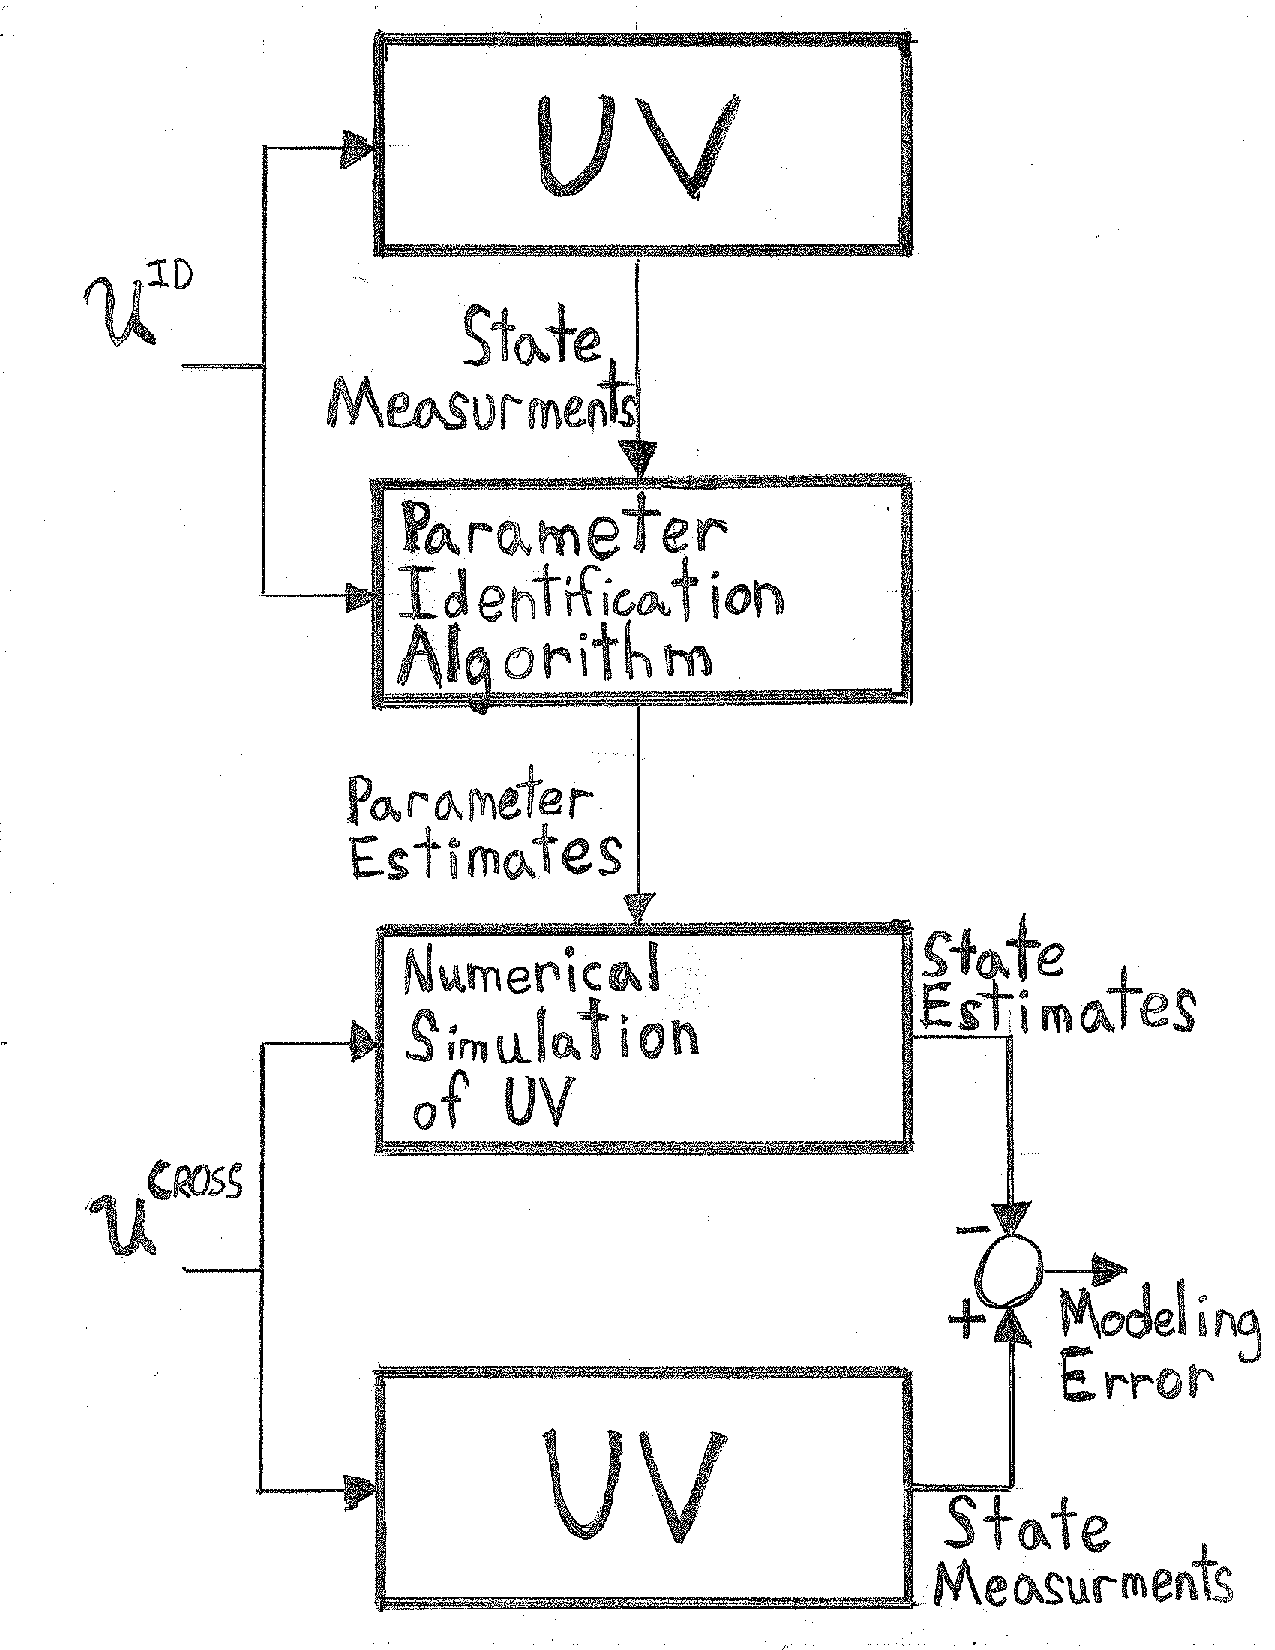
\includegraphics[width=50mm]{./pres/images/blockDiaSketch}
% %           \end{center}
% %         \end{figure}
% %       \end{center}    
% %       }
% %   \end{columns} 

% \end{frame}




%\begin{frame}{Instability Indicators: What Does Parameter Estimate Instability Look Like?}
\begin{frame}{Expt A: AMBC {\it failure }Experimental Evaluation}

\begin{itemize}
\item<1->\alert<1-4>{Problem 1:} %{Indicator 1:}  
 When initialized to
  physically realistic values, parameters adapt to physically
  unrealistic values.
\item<2-4>Consider the initial and final parameter estimates from an
  experiment where AMBC tracks a 6 DOF reference trajectory:
\begin{itemize}
\item<3-4> Most parameter estimates oscillate around initial values. (That's good)
\item<4>$\hat{m}_4(t)$ and $\hat{m}_5(t)$ adapted towards negative values.  (That's bad)
\end{itemize}
\item<5->\alert<5->{Problem 2:} %{Indicator 2:} 
Parameter estimates do
  not display asymptotic behavior.
\begin{itemize}
\item<6->$\hat{m}_4(t)$ and $\hat{m}_5(t)$ show no signs of asymptotic
  behavior.
\end{itemize}
\end{itemize}


\alt<1>{\vspace*{45mm}}{
\alt<1-5>{%\small

\begin{table}[htbp]
%\ssp
%\caption{Mass and Drag Parameters Identified During Unstable Parameter Adaptation}
\begin{center}
\begin{tabular}{c|cccc}
 & $m_i(t_o)$ & $m_i(t_f)$ & $d_i(t_o)$ & $d_i(t_f)$ \\ \hline
Trans X DOF & 583 {\it kg} & 583 {\it kg}& -1245 {\it $\frac{\text{N}~\text{s}^2}{\text{m}^2}$}& -1005 {\it $\frac{\text{N}~\text{s}^2}{\text{m}^2}$}\\
Trans Y DOF & 873 {\it kg} & 769 {\it kg}& -1426 {\it $\frac{\text{N}~\text{s}^2}{\text{m}^2}$}& -1400 {\it $\frac{\text{N}~\text{s}^2}{\text{m}^2}$}\\
Trans Z DOF & 1021 {\it kg} & 1031 {\it kg}& -3060 {\it $\frac{\text{N}~\text{s}^2}{\text{m}^2}$}& -3039 {\it $\frac{\text{N}~\text{s}^2}{\text{m}^2}$}\\
Angular X DOF & \alert<4>{103.5 {\it kg $\text{m}^2$}} & \alert<4>{-1.348 {\it kg $\text{m}^2$}} & -728.4 {\it N $\text{s}^2$}& -761.5  {\it N $\text{s}^2$}\\
Angular Y DOF & \alert<4>{137.1 {\it kg $\text{m}^2$}} & \alert<4>{42.5 {\it kg $\text{m}^2$}} & -769.1  {\it N $\text{s}^2$}& -681.4  {\it N $\text{s}^2$}\\
Angular Z DOF & 106.4 {\it kg $\text{m}^2$} & 41 {\it kg $\text{m}^2$} & -376.2  {\it N $\text{s}^2$}& -393.3  {\it N $\text{s}^2$}\\
\end{tabular}
\end{center}
\vskip9pt
\vskip9pt
%\label{chUV_AMBC.tb.startCloseDyn}
%\vspace*{-5mm}
\end{table}
}{
\begin{center}
\begin{figure}[htbp]
  \begin{center}
    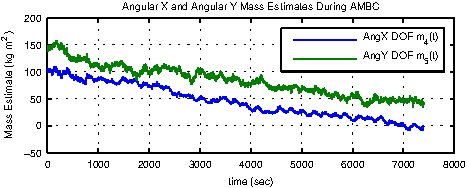
\includegraphics[width=.9\textwidth]{./chUV_AMBC/images/m4_m5_Full_Param_EstSm}
  \end{center}
%  \caption{ The time evolution of Angular X DOF and Angular Y
%    DOF mass estimates from \ac{AMBC} during 6-DOF dynamic
%    maneuvers. These mass estimates adapt to physically unrealistic
%    negative values and show no signs of asymptotic behavior.}
%  \label{chUV_AMBC.fig.m4_m5_Full_Param_Est}
%\vspace*{-5mm}
\end{figure}
\end{center}
}}

\end{frame}




%\begin{frame}{Thrust Reversals Lead to Unstable Parameter Adaptation?}
\begin{frame}{Expt B: Thrust Reversals Lead to Unstable Parameter Adaptation}

  A pitch-only AMBC experiment shows how \alert<2-3>{commanded thrust
    reversals} lead to \alt<3>{\color{blue}unmodeled thruster
    dynamics}{unmodeled thruster dynamics} which
  \alt<5>{\color{green}destabilizes}{destabilizes} parameter adaptation.

\begin{columns}
  \column{.5\textwidth} 


      \begin{center}
\alt<1>{\vspace*{30mm}}{ 
        \begin{figure}[htbp]  
          \begin{center}
            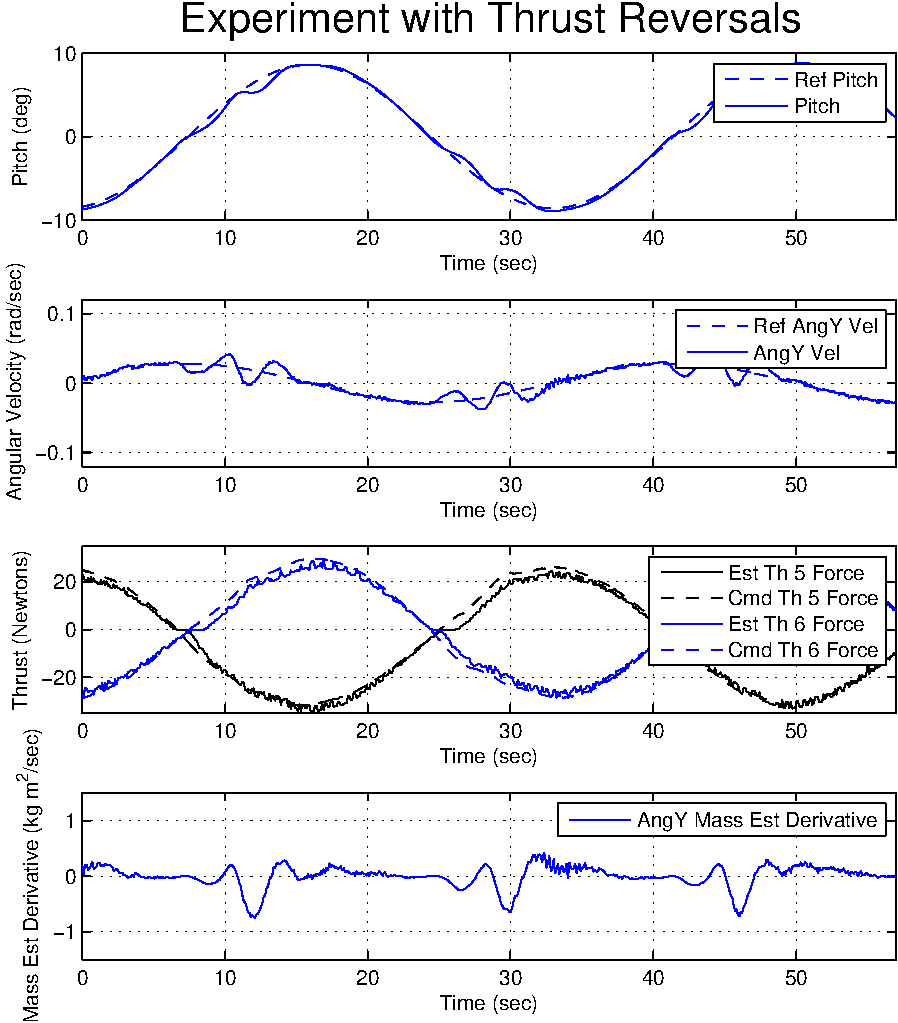
\includegraphics[width=\textwidth]{./chUV_AMBC/images/stictionErrorWithThrustReversals}
          \end{center}
        \end{figure}}
      \end{center}   

    
    \column{.5\textwidth}
      \begin{itemize}
 %     \item<1-> Commanded and Estimated Thrust shown for thrusters controlling vehicle pitch 
      \item<2-> After \alert<2-3>{thrust reversal}: \alt<3>{\color{blue}commanded thrust
        $0\text{ N}\leq u_i\leq 5$ N, estimated thrust $0$ N}{commanded thrust
        $0\text{ N}\leq u_i\leq 5$ N, estimated thrust $0$ N}
    \item<4-> AMBC interprets position and velocity deviations as the
      pitch mass estimate is too large
    \item<5->Pitch mass estimate update law has \alt<5>{\color{green}negative
        spike}{negative spike}
       \item<6->Pitch mass estimate adapts to physically unrealistic value
      \end{itemize} 
    
      \begin{center}
\alt<1-5>{\vspace*{15mm}}{\begin{figure}[htbp]  
          \begin{center}
            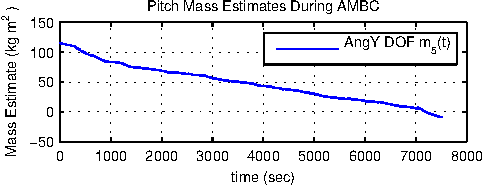
\includegraphics[width=\textwidth]{./pres/images/m5_Thrust_Rev_Param_EstSm}
          \end{center}
        \end{figure}}
      \end{center}    
      
  \end{columns} 


\end{frame}

\begin{frame}{Expt C: Stable Parameter Adaptation Without Thrust Reversals}
  For pitch-only AMBC experiment \alert<2-3>{without commanded thrust
    reversals} \alt<3>{\color{green}parameter adaptation is
    stable}{parameter adaptation is stable}.

\begin{columns}
  \column{.5\textwidth} 
 
      \begin{center}
\alt<1>{\vspace*{50mm}}{ 
        \begin{figure}[htbp]  
          \begin{center}
            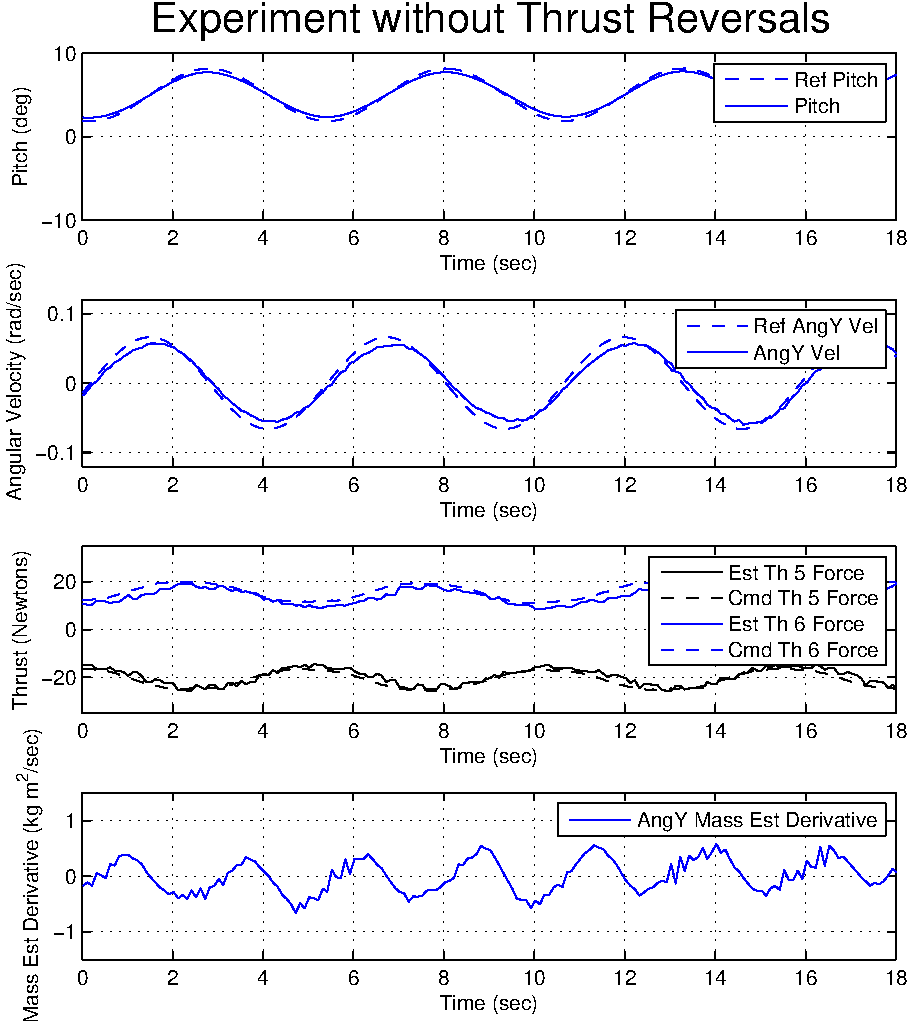
\includegraphics[width=\textwidth]{./chUV_AMBC/images/stictionErrorWoThrustReversals}
          \end{center}
        \end{figure}}
      \end{center}    

    
    \column{.5\textwidth}
      \begin{itemize}
 %     \item<1-> Commanded and Estimated Thrust shown for thrusters controlling vehicle pitch 
      \item<2->\alert<2>{No thrust reversals}
      \item<3->Without thrust reversals, velocity and position
        deviations and negative spike in the pitch mass estimate
        update law \alt<3>{\color{green}do not occur}{do not occur}
       \item<4->Pitch mass adaptation stable
      \end{itemize} 
    
      \begin{center}
\alt<1-3>{\vspace*{15mm}}{\begin{figure}[htbp]  
          \begin{center}
            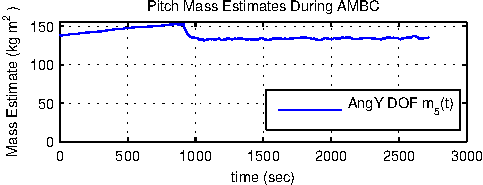
\includegraphics[width=\textwidth]{./pres/images/m5_Thrust_No_Rev_Param_EstSm}
          \end{center}
        \end{figure}}
      \end{center}    
      
  \end{columns} 


\end{frame}


\begin{frame}{Unmodeled Thruster Dynamics and Two-Step AMBC}

\begin{itemize}
%\item<1-> JHU ROV control system uses {\it steady-state} assumptions when
%  calculating thruster commands; a common assumption in UV control
%  systems.
%\item<2-> The data suggests thruster dynamics unmodeled by {\it
%    steady-state} models cause unstable parameter adaptation
%  exclusively in the pitch and roll DOF.
\item<1-> The data suggests unmodeled thruster dynamics during thrust
  reversals cause unstable parameter adaptation for parameters
  associated in the pitch and roll DOF.
\item<2-> The effects of unmodeled thruster dynamics are the same on
  buoyancy and mass estimate adaptation; this allows simultaneous
  unstable adaptation in both parameters.
\item<3-> Separately identifying mass and buoyancy parameters
  \alert<4>{COULD} prevent unstable pitch and roll parameter
  adaptation.
\item<5-> Based on UV dynamic equations it is possible to divide the
  parameter estimation process into two successive experimental trials.
\item<6->\alert<6->{Two-Step AMBC}: 
\begin{itemize}
\item<6-> First step estimates buoyancy and gravitational parameters using
  quasi-static roll and pitch reference-trajectory. 
\item<6-> Second step estimates mass and drag parameters \alert<7->{for
    any reference-trajectory}.
\end{itemize}
\end{itemize}



\end{frame}



\begin{frame}{Expt C: Two-Step AMBC Parameter Adaptation is Stable}


\begin{itemize}
\item<1->Consider the initial and final parameter estimates from the second step AMBC
  algorithm tracking a 6 DOF reference trajectory:
\begin{itemize}
\item<2->All parameter estimates were initialized zero.
\item<3->All parameter estimates converge to physically realistic values (that's good!)
\item<4->In cross-validation experiment, AMBC identified models get better at
  modeling vehicle performance through the adaptation process
\end{itemize}
\end{itemize}

\alt<2->{
\alt<1-3>{
%\vskip15pt
\begin{table}[htbp]
\caption{Parameters Identified with 
     two-step AMBC during Dynamic Motion Trajectory-Tracking}
\begin{center}
\begin{tabular}{c|cccc}
 & $m_i(t_o)$ & $m_i(t_f)$ & $d_i(t_o)$ & $d_i(t_f)$ \\ \hline
Trans X DOF & \alert<2>{0.0} {\it kg}& 628 {\it kg}& \alert<2>{0.0} {\it $\frac{\text{N}~\text{s}^2}{\text{m}^2}$}& -1259 {\it $\frac{\text{N}~\text{s}^2}{\text{m}^2}$}\\
Trans Y DOF & \alert<2>{0.0} {\it kg}& 791 {\it kg}& \alert<2>{0.0} {\it $\frac{\text{N}~\text{s}^2}{\text{m}^2}$}& -1429 {\it $\frac{\text{N}~\text{s}^2}{\text{m}^2}$}\\
Trans Z DOF & \alert<2>{0.0} {\it kg}&1043 {\it kg}& \alert<2>{0.0} {\it $\frac{\text{N}~\text{s}^2}{\text{m}^2}$}& -3083 {\it $\frac{\text{N}~\text{s}^2}{\text{m}^2}$}\\
Angular X DOF & \alert<2>{0.0} {\it kg $\text{m}^2$}& \alert<3>{95.7} {\it kg $\text{m}^2$}& \alert<2>{0.0} {\it N $\text{s}^2$}& -727.1 {\it N $\text{s}^2$}\\
Angular Y DOF & \alert<2>{0.0} {\it kg $\text{m}^2$}& \alert<3>{145.3} {\it kg $\text{m}^2$}& \alert<2>{0.0} {\it N $\text{s}^2$}& -783.4 {\it N $\text{s}^2$}\\
Angular Z DOF & \alert<2>{0.0} {\it kg $\text{m}^2$}& 110.2 {\it kg $\text{m}^2$}& \alert<2>{0.0} {\it N $\text{s}^2$}& -465.6 {\it N $\text{s}^2$}\\
\end{tabular}
\end{center}
\end{table}
}{
\vspace*{3mm}
\vskip9pt
{\scriptsize
\begin{table}[htbp]
\caption{Mean Absolute Error Values Comparing Simulated and Measured Vehicle Performance for Cross-Validation Experiment}
\begin{center}
\begin{tabular}{p{1.5cm}|cccccccc}
Time of AMBC & \multicolumn{2}{c}{Angular Pose ($^\circ$)} & \multicolumn{3}{c}{Translational Velocity (m/s) }& \multicolumn{3}{c}{Angular Velocity ($^\circ$/s)} \\ 
Parameter Set & Roll & Pitch & x DOF & y DOF & z DOF & x DOF & y DOF & z DOF \\ \hline
250 sec      &  2.6 & 2.2 & 0.102  & 0.107  & 0.35  & 2.3 & 2.4 & 4.3 \\
1000 sec     &  2.2 & 1.81 & 0.048  & 0.042 & 0.138  & 1.77 & 1.48 & 3.6 \\
5000 sec     & 1.06 & 1.1 & 0.039  & 0.042  & 0.035 & 1.34 & 0.89 & 2.8 \\
\end{tabular}
\end{center}
\end{table}}
\vskip9pt
\vskip9pt
\vskip9pt
\vskip9pt
}}{\vspace*{47mm}}

\end{frame}


% \begin{frame}{Forward simulation of two-step AMBC identified models}

% \begin{columns}
%     \column{.5\textwidth}

%      \begin{center}
%         \begin{figure}[htbp]  
%           \begin{center}
%             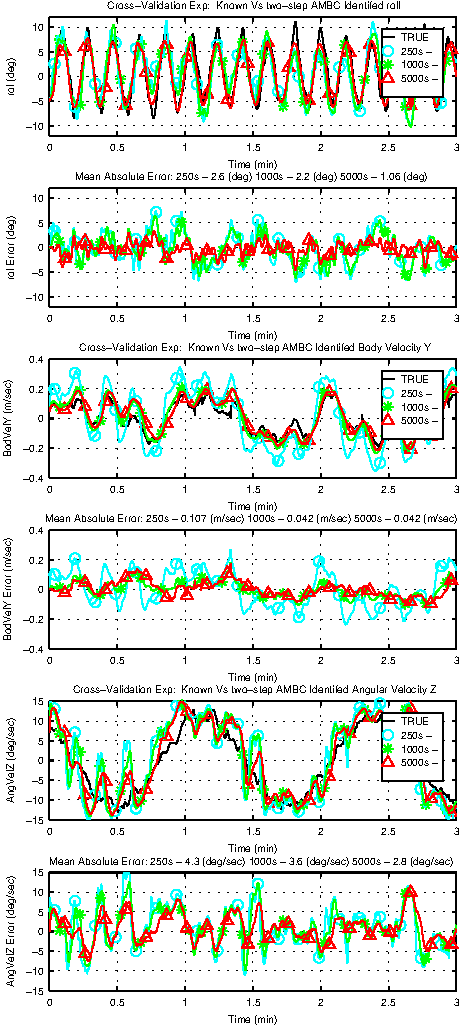
\includegraphics[width=.8\textwidth]{./chUV_AMBC/images/OLO_All}
%           \end{center}
%         \end{figure}
%       \end{center}    

%     \column{.5\textwidth}

% \begin{itemize}
% \item Experimentally measured states verses the states from numerical
%   simulations; each numerical simulation uses a model identified by
%   the two-step AMBC after a set amount of time.
% \item parameter estimates are progressively improving at modeling JHU ROV performance
% \item The states shown from simulating the ``5000
% sec'' parameter set indicate that AMBC can produce parameter estimates
% which result in accurate plant models.
% \end{itemize}

% \vskip9pt
% \vskip9pt
% \vskip9pt
% \vskip9pt
% \vskip9pt
% \vskip9pt

% \end{columns}


% \end{frame}



%\begin{frame}{Two-Step AMBC}
%
%\end{frame}





\begin{frame}{Expt C: Two-Step AMBC vs PDC Comparative Experimental Analysis}

\begin{itemize}
%\item<1->PDC tracking performance compared to second-step AMBC
%  tracking performance with the same PD gains and reference trajectory
\item<2->Mean normalized of errors vectors (MNE) for
  position and velocity
\begin{itemize}
\item<3->PDC MNE values calculated using 10 minutes of data%,  plotted in green 
\item<4->AMBC MNE values calculated for consecutive 15 minute windows%, plotted in blue
\end{itemize}
\item<5->After parameter convergence the two-step AMBC provides
$30\%$ better position tracking and $8\%$ worse velocity tracking.
\end{itemize}

\begin{center}
\begin{figure}[htbp]
  \begin{center}
    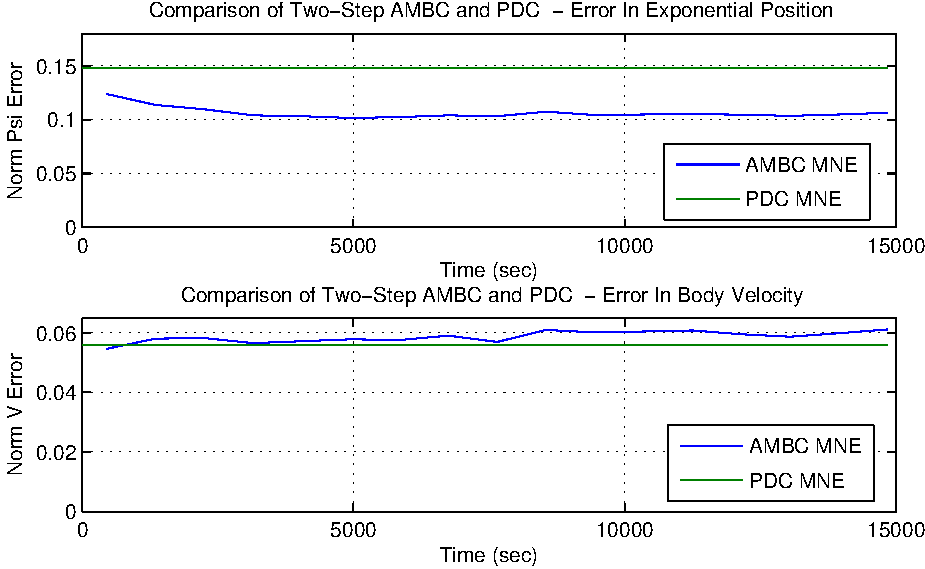
\includegraphics[width=.8\textwidth]{./chUV_AMBC/images/MNE_All}
  \end{center}
\end{figure}
\end{center}

\end{frame}



\section{Conclusion}
\subsection{Summary}


\begin{frame}[t]{Motivation}
  Recent advances in Underwater Vehicle (UV) systems have enabled
  scientists and engineers to consider complex, multifaceted UV
  missions previously thought impractical or infeasible.

\alert{Thesis Goal}: Develop improved
  {\bf state estimation}, {\bf parameter identification}, and
  {\bf control} algorithms.
%    
    \begin{columns}
      \column{.45\textwidth}
\begin{center}
      \begin{figure}[htbp]
        \begin{center}
          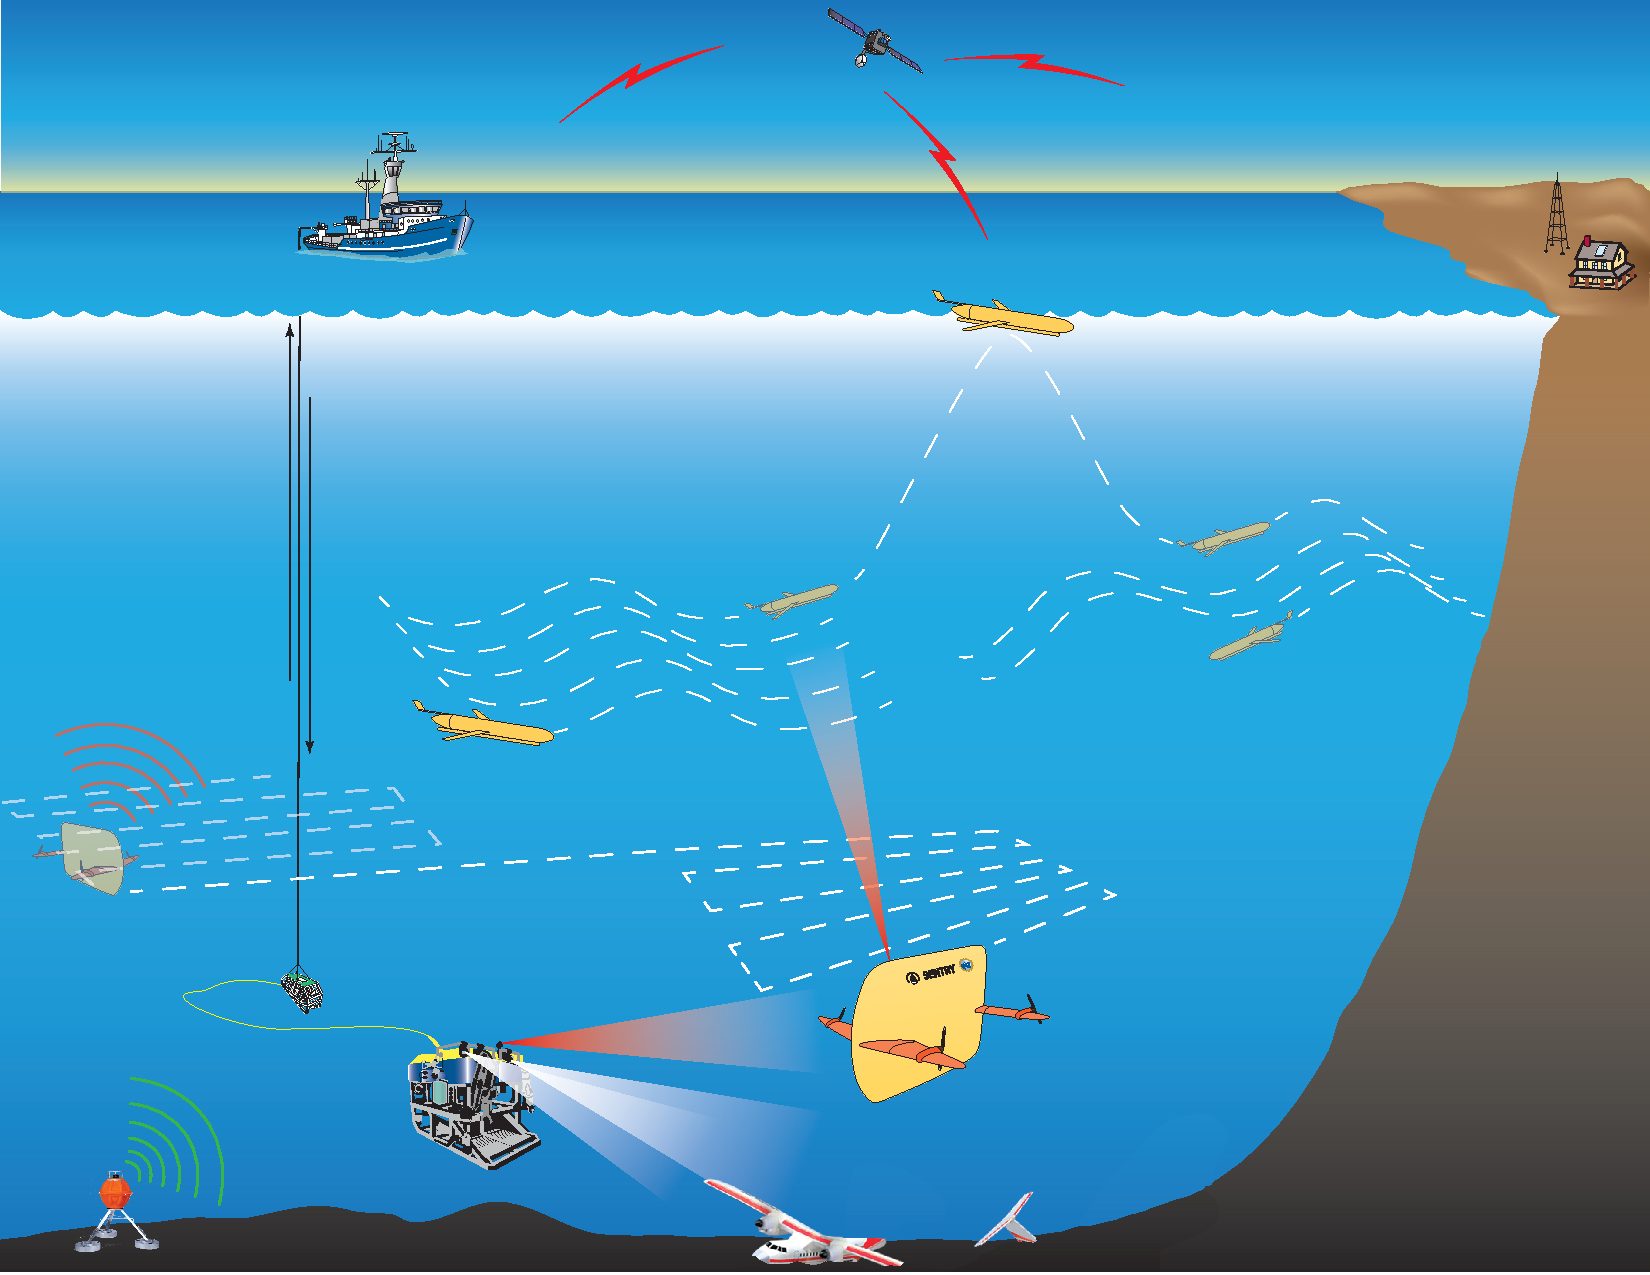
\includegraphics[width=1.1\textwidth]{./pres/images/Adaptive4}
%\caption{ Image credit: Paul Oberlander, WHOI. }
        \end{center}
      \end{figure}
    \end{center}
{\small Image credit: Paul Oberlander, WHOI.}

  \column{.55\textwidth}

  \begin{itemize}
  \item {\bf Improved State Estimation} algorithms can
    increase navigation accuracy while lowering UV cost.
  \item {\bf Improved Parameter Identification} algorithms enable
    remote operators to use forward simulation for mission planning
    and diagnose UV failure.
  \item {\bf Improved Control} algorithms enable increased precision
    of delicate or dynamic 6-degree-of-freedom
    (DOF) operation.
  \end{itemize}


 \end{columns}

\end{frame}


% \begin{frame}{Summary}
% %  Recent advances in Underwater Vehicle (UV) systems have enabled
% %  scientists and engineers to consider complex, multifacited UV
% %  missions previously thought impractical or impossible.

%   \alert{Thesis Goal}: Develop improved {\bf state estimation}, {\bf parameter
%     identification}, and {\bf control algorithms}.

% \vskip9pt    
% \vskip9pt    
% \vskip9pt    
%     \begin{columns}
%       \column{.5\textwidth}
% \alt<1>{}{    \begin{center}
%       \begin{figure}[htbp]
%         \begin{center}
%           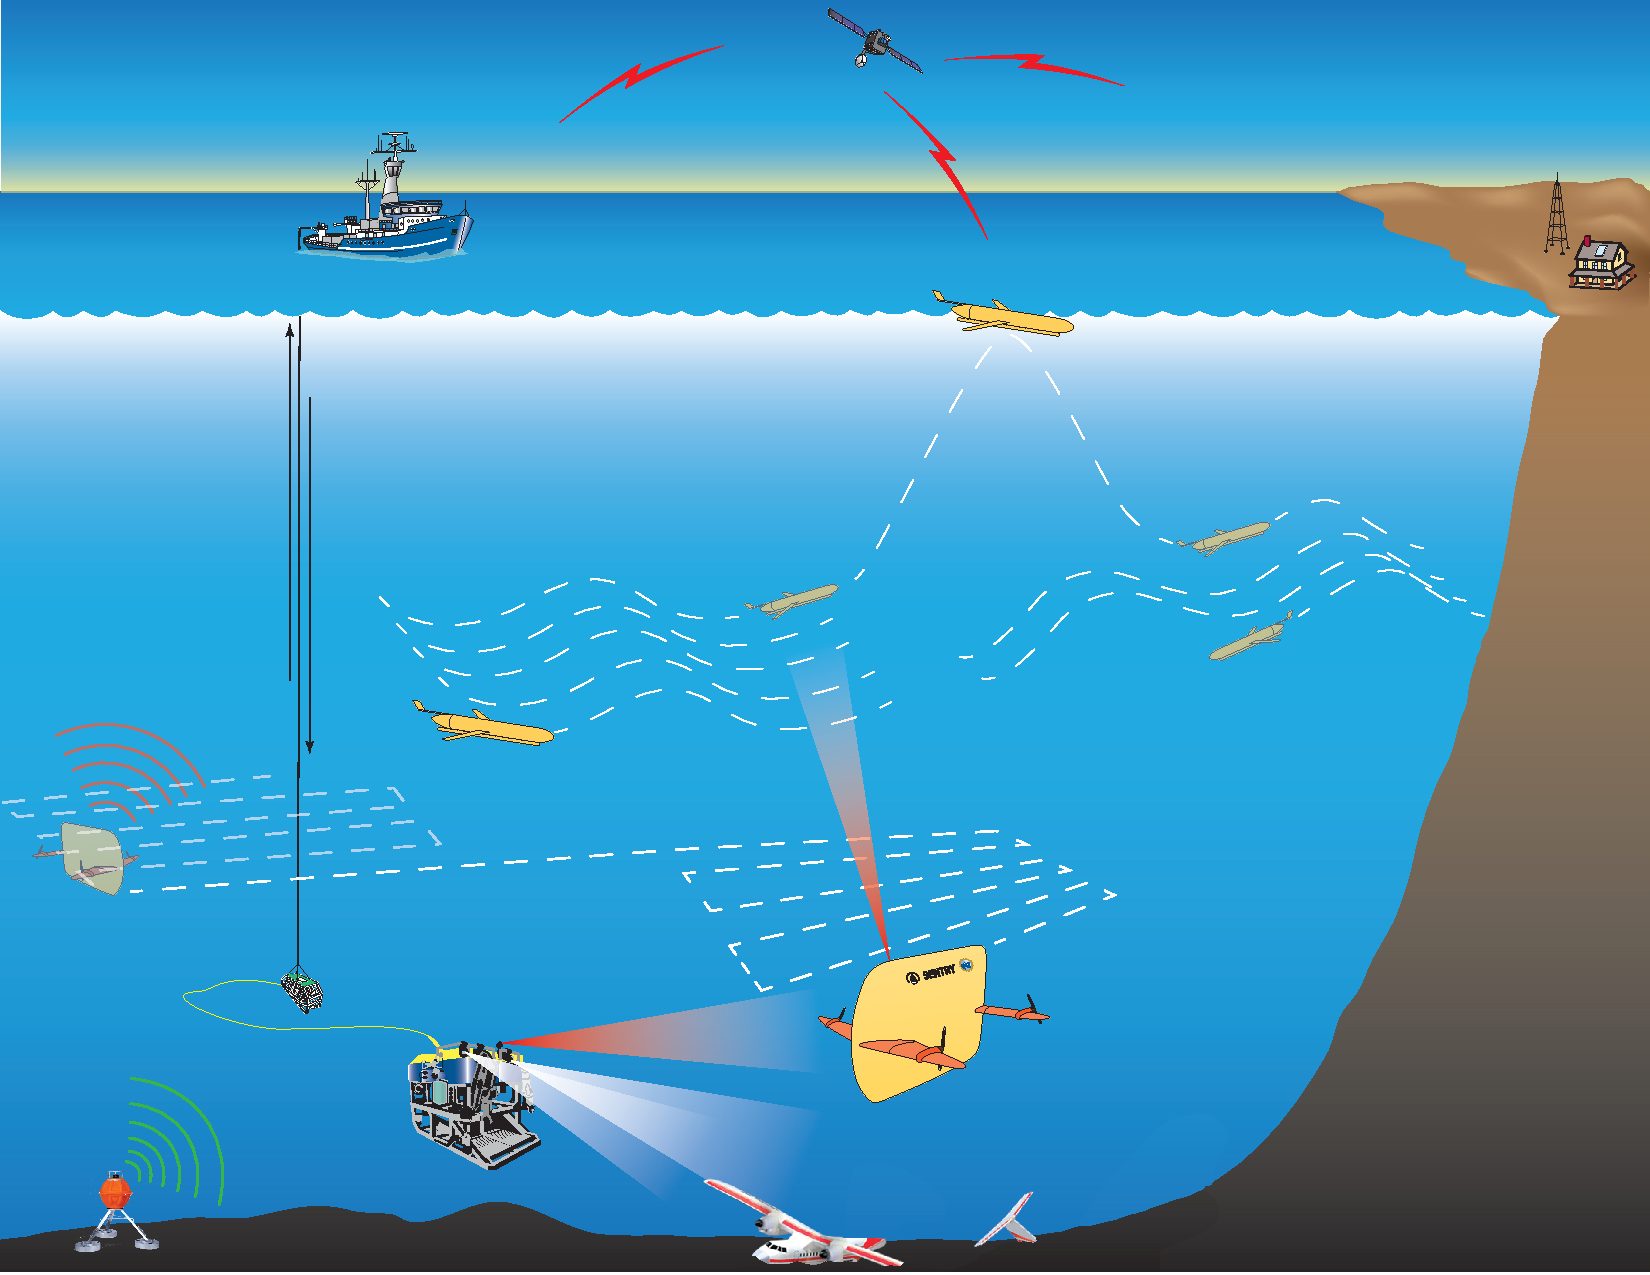
\includegraphics[width=\textwidth]{./pres/images/Adaptive4}
% %\caption{ Image credit: Paul Oberlander, WHOI. }
%         \end{center}
%       \end{figure}
%     \end{center}
% {\small Image credit: Paul Oberlander, WHOI.}}

%   \column{.5\textwidth}
% \vskip9pt
%   \uncover<2->{ The state estimation, adaptive identification, and
%     adaptive model-based control algorithms reported preform as well
%     as or better than current solutions.  
% \vskip9pt
% %They do so with while
% %    considering complicating features %such as underactuated vehicles or unmodeled thruster dynamics, which must
% %    which must be addressed before fielding such algorithms in the open ocean.
% \vskip9pt
% \vskip9pt
% \vskip9pt
% \vskip9pt}
%  \end{columns}

% \end{frame}


\subsection{Questions?}
\begin{frame}[t]{Questions?}
\begin{columns}
\column{.5\textwidth}
  \tableofcontents
\column{.5\textwidth}
  \begin{center}
\begin{figure}[htbp]  
  \begin{center}
    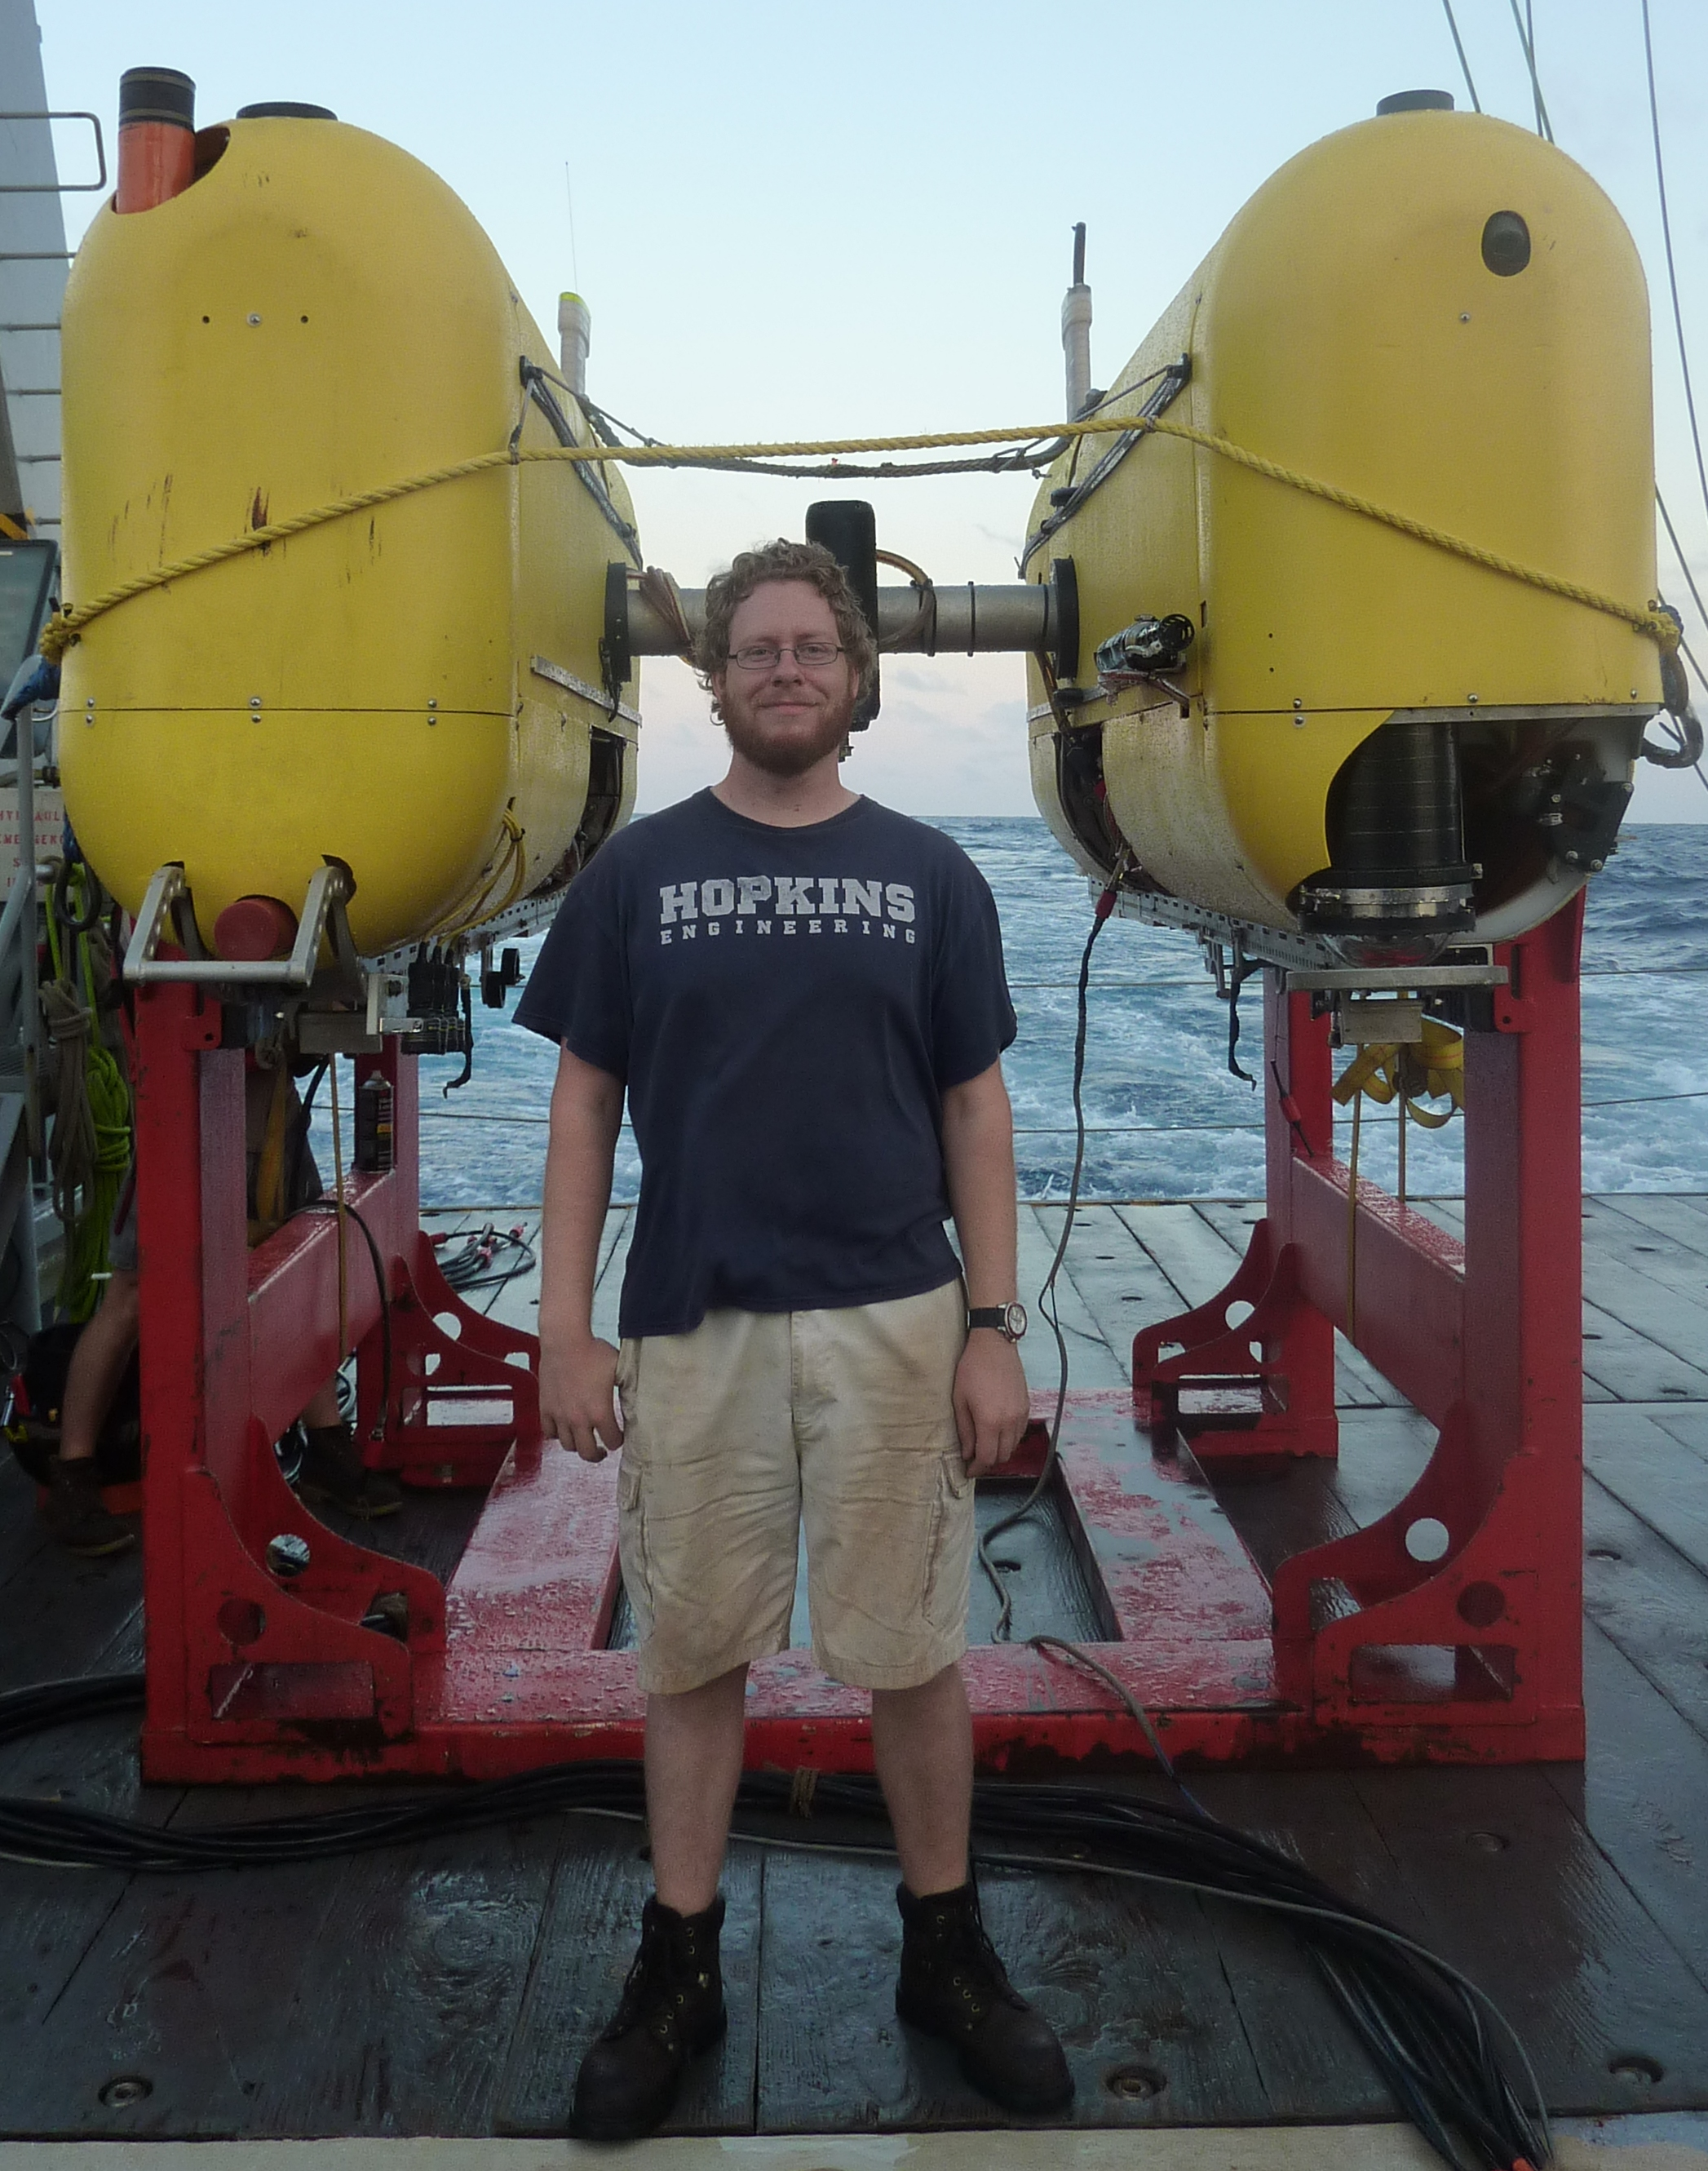
\includegraphics[width=40mm]{./pres/images/tophNereus}
  \end{center}
  \caption{McFarland and Nereus (WHOI) during field deployment in 2011.}
\end{figure}
\end{center}
\end{columns}

\end{frame}

%-------------------------------------------------------------------
%2013-04-23  toph  FOR NOW COMMENTED OUT ADDITIONAL SLIDES SECTIONS

% \section{Additional Slides}

% \subsection{AID Stability Analysis}

% \begin{frame}[t]{Rigid Body Model}
%   \begin{align} 
%     \uncover<1>{\dot{R}(t)}&\uncover<1>{=R(t)\mathcal{J}(\omega(t))}
%     \nonumber \\
%     I\dot{\omega}(t)&=\mathcal{J}(I\omega(t))\omega(t)
%     \uncover<1>{+\left(\sum_{i=1}^3 |\omega_i|C_i
%     \right)\omega(t)+\mathcal{J}(b)R(t)^T e_3}+u(t)
%     \nonumber 
%  \end{align}

%  \begin{itemize}
%    \item<2-> Standard Second Order Rotating Rigid Body System 
%    \item<3-> Typically used to model satellites
%    \item<4-> We first developed an Adaptive Identifier for this system first
%  \end{itemize}

% \end{frame}


% \begin{frame}{Rigid Body Adaptive Identification}

%   \begin{columns}
%     \column{.32\textwidth}

%     Error Coordinates:
%     \begin{align}
%       \Delta\omega(t)&=\hat{\omega}(t)-\omega(t)  \nonumber \\
%       \Delta I(t)&=\hat{I}(t) - I                 \nonumber
%     \end{align}
    
%     System:
%     \begin{equation*}
%       \dot{\omega} =I^{-1}\left(\mathcal{J}(I\omega)\omega+u\right) 
%     \end{equation*}
    
%     Adaptive Identifier:
%     \begin{align}
%       \dot{\hat{\omega}}=&\hat{I}^{-1}\left(
%         \mathcal{J}(\hat{I}\omega)\omega
%         + u\right) - a \Delta \omega    \nonumber \\
%       \dot{\hat{I}}=&-\frac{1}{2}\left(\psi_1 \omega^T +\omega
%         \psi_1^T\right)
%       \nonumber \\
%       &+\frac{1}{2}\left(\Delta\omega \psi_2^T+\psi_2
%         \Delta\omega^T\right)\only<5>{.}  \nonumber
%     \end{align}
    
%     \pause
    
%     \column{.68\textwidth}
%     \temporal<3>
%     {with the following constraints:
%       \begin{itemize}
%       \item $u(t)$ and $\omega(t)$ bounded by assumption
%       \item $a\in\mathbb{R}_+$
%       \item $\psi_1=\mathcal{J}(\omega)\Delta \omega$
%       \item
%         $\psi_2=\hat{I}^{-1}\left(\mathcal{J}\left(\hat{I}\omega\right)
%           \omega +u\right)$
%       \item $\hat{I}(t_0)$ is SPD
%       \item $\hat{\omega}(t_0)=\omega(t_0)$
%       \item $\exists \epsilon \in \mathbb{R}_+$ such that $\|\Delta
%         I(t_0)\|_F+\epsilon \leq \lambda_3$
%       \end{itemize}
      
%     }{ 
      
%       %\color{green}{Lyapunov Stability Proof Outline}
%       %Lyapunov Stability Proof Outline
%       Error Dynamics:
%       \begin{align}
%         \dot{\Delta I}&=-\frac{1}{2}\left(\psi_1 \omega^T +\omega
%           \psi_1^T -\Delta\omega \psi_2^T-\psi_2 \Delta\omega^T\right)
%         \nonumber \\
%         \dot{\Delta \omega}&=-I^{-1}\left(a I
%           \Delta\omega+\mathcal{J}(\omega)\Delta I \omega +\Delta I
%           \psi_2\right) 
%         \nonumber
%       \end{align}

%       Lyapunov Equation:
%       \begin{align}
%         V(t)&=\frac{1}{2}\left(\Delta \omega^{T} I \Delta \omega +
%           \tr\left(\Delta I \Delta I^{T}\right)\right)
%         \nonumber \\
%         \dot{V}(t)&=-a\Delta\omega^{T}I\Delta\omega \nonumber
%       \end{align}

%       \begin{itemize}
%       \item $V(t)$ positive definite, radially unbounded 
%       %\item $V(t)$ 
%       \item $V(t)=0$ $\Leftrightarrow$ $\Delta \omega=\vec{0}$,
%         $\Delta I=0_{3\times 3}$
%       \item $\dot{V}(t)$ negative semi-definite
%       \end{itemize}
%     }{ 

%       With these conditions and Lyapunov stability analysis we prove
%       the estimated angular velocity is asymptotically stable
%       (i.e. $\lim_{t\to \infty}\Delta \omega=\vec{0}$) and the
%       estimated inertia tensor will converge to a constant value
%       (i.e. $\lim_{t\to \infty}\Delta \dot{I}=0_{3\times3}$). These
%       limits imply that \alert<5->{parameter estimates converge to
%         values that provide input-output behavior identical to that of
%         the actual experimental plant for the given input $u(t)$.}

%     }
%   \end{columns}
% \end{frame}


% \begin{frame}{UUV Adaptive Identification}

%   System and Adaptive Identifier:
%   \begin{equation*}
%     \dot{\omega}=I^{-1}\left(\mathcal{J}(I\omega)\omega+\left(\sum_{i=1}^3 |\omega_i|C_i
%       \right)\omega+\mathcal{J}(b)R^T e_3+u\right)
%   \end{equation*}
  
%   \vskip0pt plus.5fill
  
%   \begin{align}
%     \dot{\hat{\omega}}=&\hat{I}^{-1}\left( \mathcal{J}(\hat{I}\omega)\omega
%       +\sum_{i=1}^3 |\omega_i|\hat{C}_i\omega+\mathcal{J}(\hat{b})R^T e_3
%       + u\right)- a \Delta \omega   \nonumber \\
%     \dot{\hat{I}}=&-\frac{\gamma_1}{2}\left(\psi_1 \omega^T 
%       +\omega \psi_1^T-\Delta\omega \psi_3^T-\psi_3 \Delta\omega^T\right)\nonumber\\
%     \dot{\hat{C_i}}=&-\gamma_2|\omega_i|\Delta\omega \omega^T
%     \nonumber \\
%     \dot{\hat{b}}=&-\gamma_3\mathcal{J}(R^T e_3)\Delta\omega
%     \nonumber 
%   \end{align}
  
%   With constraints and a stability analysis mirroring those just
%   presented, \alert<2->{we can again guarantee plant parameter estimates
%     converge to values that provide input-output behavior identical to
%     that of the actual experimental plant for the given input $u(t)$.}
  
% \end{frame}

% \subsection{Analysis: Identification Exp}

% \begin{frame}{Analysis: Parameter Identification Experiment}

% \begin{table}[htbp]
% \caption{Mean Absolute Error Values for Identification Experiment.}
% \begin{center}
% \begin{tabular}{p{1.5cm}|ccccc}
% & \multicolumn{2}{c}{Angular Pose} & \multicolumn{3}{c}{Angular Velocity} \\ 
% Parameter Set & Roll & Pitch & x DOF & y DOF & z DOF \\ \hline
% AID  & 3.44$^\circ$ & 2.06$^\circ$ & 4.80$^\circ$/s & 1.99$^\circ$/s & 4.03$^\circ$/s \\
% LS   & 2.08$^\circ$ & 1.76$^\circ$ & 2.45$^\circ$/s & 2.19$^\circ$/s & 5.05$^\circ$/s \\
% INIT & 14.8$^\circ$ & 17.1$^\circ$ & 8.83$^\circ$/s & 10.7$^\circ$/s & 6.32$^\circ$/s \\
% \end{tabular}
% \end{center}
% \end{table}

% \end{frame}

% \begin{frame}[t]{Questions?}
% \begin{columns}
% \column{.5\textwidth}
%   \tableofcontents
% \column{.5\textwidth}
%   \begin{center}
% \begin{figure}[htbp]  
%   \begin{center}
%     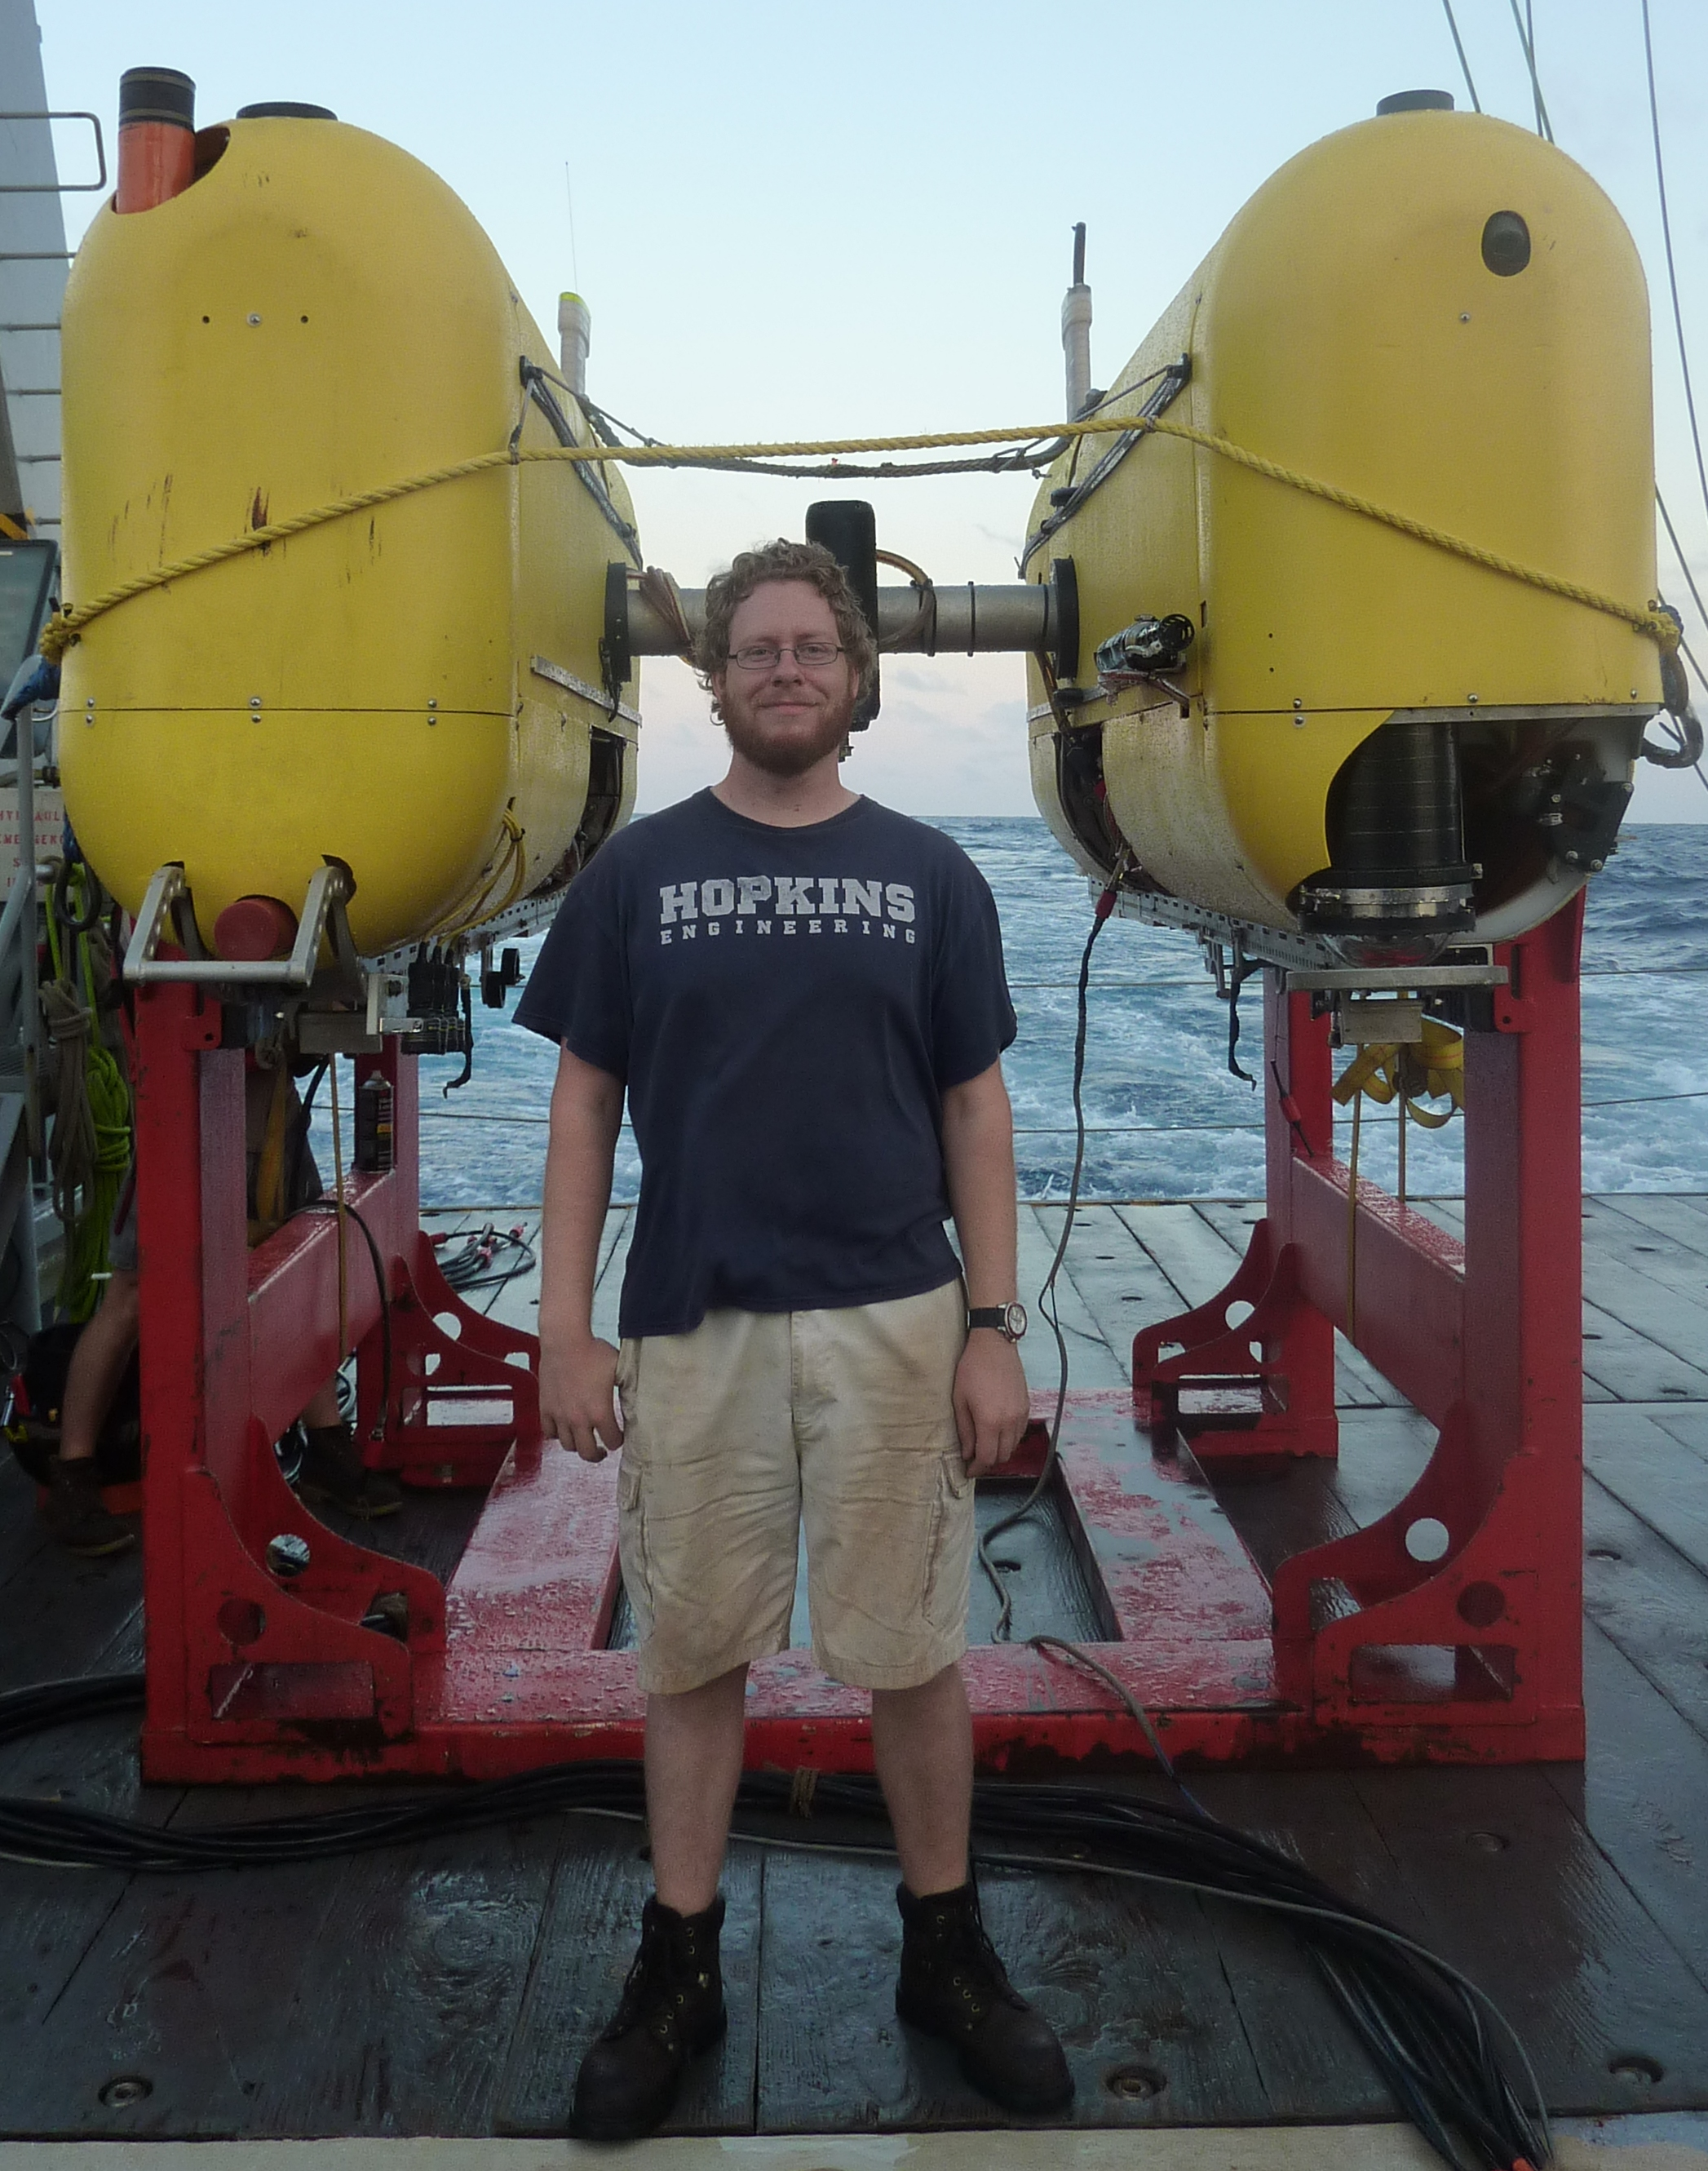
\includegraphics[width=40mm]{./pres/images/tophNereus}
%   \end{center}
%   \caption{McFarland and Nereus (WHOI) during field deployment in 2011.}
% \end{figure}
% \end{center}
% \end{columns}
% \end{frame}



% All of the following is optional and typically not needed. 
% \appendix
% \section<presentation>*{\appendixname}
% \subsection<presentation>*{For Further Reading}

% \begin{frame}[allowframebreaks]
%   \frametitle<presentation>{For Further Reading}
    
%   \begin{thebibliography}{10}
    
%   \beamertemplatebookbibitems
%   % Start with overview books.

%   \bibitem{Author1990}
%     A.~Author.
%     \newblock {\em Handbook of Everything}.
%     \newblock Some Press, 1990.
 
    
%   \beamertemplatearticlebibitems
%   % Followed by interesting articles. Keep the list short. 

%   \bibitem{Someone2000}
%     S.~Someone.
%     \newblock On this and that.
%     \newblock {\em Journal of This and That}, 2(1):50--100,
%     2000.
%   \end{thebibliography}
% \end{frame}


\end{document}


